\documentclass[11pt,addpoints,answers]{exam}
% 1. 加载所有必需包(按依赖顺序排列,避免冲突)
\usepackage[margin=1in]{geometry}
\usepackage{amsmath,amssymb}       % 数学符号与公式
\usepackage{booktabs}              % 表格美化
\usepackage{array}                 % 表格扩展
\usepackage{enumitem}              % 列表控制
\usepackage[many]{tcolorbox}       % 自定义盒子(必须加载many选项)
\usepackage{graphicx}              % 图片插入
\usepackage{caption}               % 图片/表格标题
\usepackage{tikz}                  % 绘图
\usetikzlibrary{calc}              % tikz坐标计算
\usepackage{multicol}              % 多列排版
\usepackage{float}                 % 固定图片位置
\usepackage{bm}                    % 加粗数学符号
\usepackage{hyperref}              % 超链接(最后加载,避免冲突)
\usepackage{listings}              % 代码高亮
\usepackage{subcaption}            % 子图环境
\usepackage{pdfpages}			   % 插入PDF文件


\title{\textbf{Machine Learning Homework Solution}}
\author{Yuecheng Han 524531910029}
\date{\today}

% 2. 核心命令定义(修复tcolorbox和子问题环境)
% 2.0 向量和矩阵命令(加粗)
\newcommand{\xv}{\mathbf{x}}
\newcommand{\yv}{\mathbf{y}}
\newcommand{\wv}{\mathbf{w}}
\newcommand{\vv}{\mathbf{v}}
\newcommand{\uv}{\mathbf{u}}
\newcommand{\thetav}{\boldsymbol{\theta}}
\newcommand{\Xv}{\mathbf{X}}
\newcommand{\Dc}{\mathcal{D}}
\newcommand{\Omegav}{\boldsymbol{\Omega}}

% section question command
\newcommand{\sectionquestion}[1]{\section*{#1}}

% subparts environment is already defined by exam class, no need to redefine
% 2.1 自定义答案框(正确语法,无多余空格)
\newtcolorbox{answer_box}[1][]{
	enhanced,
	nobeforeafter,
	colback=white,
	title={#1},  % 修复:title参数用{}包裹,避免解析错误
	box align=top,
	boxrule=0.8pt,
	colframe=black!70,
	fontupper=\small,
	height=3cm,
	#1
}

% 自定义学生答案框
\newtcolorbox{your_solution}[1][]{
	enhanced,
	nobeforeafter,
	colback=white,
	box align=top,
	boxrule=0.8pt,
	colframe=black!70,
	fontupper=\small,
	#1
}

% 2.2 子问题环境(基于enumerate,避免与exam类冲突)
\newcounter{subq}        % 子问题计数器
\renewcommand{\thesubq}{(\alph{subq})}  % 子问题编号:(a),(b)...
\newenvironment{subquestions}{
	\setcounter{subq}{0}%  % 每次开始subquestions时重置计数器
	\begin{enumerate}[
		label=\thesubq,
		leftmargin=*,
		align=left,
		itemsep=6pt
		]
	}{
	\end{enumerate}
}
\newcommand{\subquestion}{\refstepcounter{subq}\item}  % 子问题命令

% 2.3 复选框样式(全局统一,适配exam类)
\CorrectChoiceEmphasis{}
\checkedchar{\blacksquare}
\checkboxchar{$\Box$}

% 2.4 缩写命令(避免重复代码)
\newcommand{\sall}{\textbf{Select all that apply: }}
\newcommand{\sone}{\textbf{Select one: }}

% 2.5 配置listings包用于代码显示
\lstset{
	basicstyle=\ttfamily\small,
	breaklines=true,
	columns=fullflexible,
	keepspaces=true,
	showstringspaces=false,
	frame=single,
	tabsize=4
}

% 3. 重置part计数器(解决标签重复)
\renewcommand{\thepart}{\arabic{part}}  % part编号为阿拉伯数字,避免与其他计数器冲突
\renewcommand{\partlabel}{\thepart.}



\begin{document}
	\section*{Problem 1 : Coding}
	\label{sec:pseudocode}
	
	The following questions should be completed before you start the programming component of this assignment. Assume the \texttt{dtype}s of all \texttt{ndarray}s are \texttt{np.float64}. Vectors are 1D \texttt{ndarray}s.
	
	\textbf{Note:} These questions require understanding of NumPy broadcasting. Please refer to the NumPy documentation for broadcasting concepts and rules: \url{https://numpy.org/doc/stable/user/basics.broadcasting.html}
	
	\begin{enumerate}[label=\alph*), itemsep=10pt]
		\item[(1)] \sall Given a data matrix $\Xv \in \mathbb{R}^{N \times M}$ and a weight vector $\vv \in \mathbb{R}^M$. The following code snippet computes a result vector $\uv \in \mathbb{R}^N$ where each component $u_i$ represents the weighted sum of the $i$-th row of $\Xv$ with weights given by $\vv$:
		\begin{lstlisting}[language=Python,escapechar=@]
# X and v are numpy ndarrays
# X has shape (N, M), v has shape (M,)
u = np.zeros(N)
for row_idx in range(N):
	for col_idx in range(M):
		u[row_idx] += X[row_idx, col_idx] * v[col_idx]
		\end{lstlisting}
		\vspace*{-2.5mm}
		Select all equivalent NumPy operations that compute the same output:
		
		{%
				\checkboxchar{$\Box$} \checkedchar{$\blacksquare$}
			\begin{checkboxes}
				\CorrectChoice \texttt{u = X @ v}
				\choice \texttt{u = v @ X}
				\CorrectChoice \texttt{u = np.matmul(X, v)}
				\choice \texttt{u = np.matmul(v, X)}
				\choice \texttt{u = X * v}
				\choice \texttt{u = v * X}
				\CorrectChoice \texttt{u = np.dot(X, v)}
				\choice \texttt{u = np.dot(v, X)}
				\choice None of the above.
			\end{checkboxes}
		}
		
		
		
		\item[(2)] Suppose we have a feature matrix $\Xv \in \mathbb{R}^{N \times M}$ and a coefficient vector $\wv \in \mathbb{R}^N$. Define a matrix $\Omegav$ computed as follows: $\Omegav = \sum_{i=0}^{N-1} w_i \left(\xv_i - \overline{\xv_i}\right) \left(\xv_i - \overline{\xv_i}\right)^T$, where $\xv_i \in \mathbb{R}^{M}$ represents the $i$-th \textit{row} of $\Xv$ (expressed as a \textit{column} vector), $\overline{\xv_i} \in \mathbb{R}$ denotes the average value of all elements in $\xv_i$, and $w_i \in \mathbb{R}$ is the $i$-th component of $\wv$ (for $i \in \{0, 1, \cdots, N-1\}$). In the following questions, let \texttt{X} and \texttt{w} represent $\Xv$ and $\wv$ respectively, where \texttt{X.shape == (N, M)} and \texttt{w.shape == (N,)}. %\textbf{You must use NumPy and vectorize your code for full credit.} Do \textit{not} use functions which are essentially wrappers for Python loops and provide little performance gain, such as \texttt{np.vectorize}.
		\begin{enumerate}[label=(\roman*), leftmargin=*]
			
			\item \sone Identify the correct line(s) of Python code that generates a matrix where each row $i$ equals $\left(\xv_i - \overline{\xv_i}\right)^T$ (i.e., the $i$-th row of $\Xv$ after subtracting its row-wise mean).
			
			{%
				\checkboxchar{$\Box$} \checkedchar{$\blacksquare$}
				\begin{checkboxes}
					\choice \texttt{(X - np.mean(X, axis=0)).T}
					\CorrectChoice \texttt{X - np.mean(X, axis=1, keepdims=True)}
					\choice \texttt{X - np.mean(X, axis=0, keepdims=True)}
					\choice \texttt{X - np.expand\_dims(np.mean(X, axis=1), 1)}
					\choice None of the above.
				\end{checkboxes}
			}
			
			
			\item \sone Let \texttt{M} store the output from part (i). Which line(s) of code correctly evaluate $\Omegav$ using \texttt{M}? \\
			
			{
				\checkboxchar{$\Box$} \checkedchar{$\blacksquare$}
				\begin{samepage}
					\begin{checkboxes}
						\CorrectChoice \texttt{np.matmul(w * M.T, M)}
						\choice \texttt{np.matmul(w * M, M.T)}
						\choice \texttt{np.dot(w * M, M.T)}
						\choice \texttt{w * np.dot(M.T, M)}
						\choice None of the above.
					\end{checkboxes}
				\end{samepage}
			}
			
			
		\end{enumerate}
		
	\end{enumerate}
	\section*{Problem 2 : Linear Regression}
	
	\begin{enumerate}
		\item[1.] 
		\begin{enumerate}[label=\alph*), itemsep=10pt]
			\item[(1)] You are given the following training data for a regression task:
			\begin{table}[H]
				\centering
				\begin{tabular}{llllll}
					$x$ & 7.0 & 3.0 & 5.0 & 2.0 & 6.0 \\
					$y$ & 2.0 & 1.0 & 2.0 & 0.0 & 3.0
				\end{tabular}
				\caption{Regression Dataset} \label{tab:reg7_data}  % 唯一标签
			\end{table}
			Denote $\bm{x}$ as the feature vector and $\bm{y}$ as the target vector. We apply gradient descent optimization to fit a linear model with cost function $J(w, b) = \dfrac{1}{N}\sum\limits_{i=1}^N (wx_i + b - y_i)^2$, where $N$ represents the sample count, $w$ denotes the slope parameter, and $b$ denotes the bias term.
			
			\textbf{Note:} While demonstrating your calculation steps is optional, we encourage you to show your work for potential partial credit if your final answer contains errors.
			
			\begin{subquestions}
				\subquestion Suppose we set the initial slope parameter to $3.0$ and the initial bias term to $0.0$. Compute the derivative of the cost function with respect to the slope $w$ using the complete dataset during the initial gradient descent iteration. 
				\\ \textbf{Round to 4 decimal places after the decimal point.}
				
				\begin{answer_box}[title=Gradient:,height=2cm,width=6cm]
					% 答案区域
					$129.6000$
				\end{answer_box}
				
				\begin{answer_box}[title=Work,height=6cm]
					$\nabla_w J = \frac2N\sum_{i=1}^N (wx_i + b - y_i)x_i$

					Let $N=5$, $w=3.0$, $b=0.0$, and input the data points:

					$\nabla_w J = \frac25\left((3*7.0 + 0.0 - 2.0)*7.0 + (3*3.0 + 0.0 - 1.0)*3.0 + \right.$\\
					$\left.(3*5.0 + 0.0 - 2.0)*5.0 + (3*2.0 + 0.0 - 0.0)*2.0 + (3*6.0 + 0.0 - 3.0)*6.0\right)$\\
					$= 129.6000.$

				\end{answer_box}
				
				\clearpage
				
				\subquestion Calculate the derivative of the cost function with respect to the bias parameter $b$, evaluated across the entire training set for the first iteration.
				
				\begin{answer_box}[title=Gradient:,height=2cm,width=6cm]
					% 答案区域
					$24.4000$
				\end{answer_box}
				
				\begin{answer_box}[title=Work,height=8cm]
					$\nabla_b J = \frac2N\sum_{i=1}^N (wx_i + b - y_i)$

					Let $N=5$, $w=3.0$, $b=0.0$, and input the data points:

					$\nabla_b J = \frac25\left((3*7.0 + 0.0 - 2.0) + (3*3.0 + 0.0 - 1.0) + \right.$\\
					$\left.(3*5.0 + 0.0 - 2.0) + (3*2.0 + 0.0 - 0.0) + (3*6.0 + 0.0 - 3.0)\right)$\\
					$= 24.4000.$
				\end{answer_box}
				
				\subquestion Using a step size of $0.01$, execute one iteration of the gradient descent algorithm. Report the updated values of both the slope and bias parameters following this update step. 
				\\ \textbf{Round to 4 decimal places after the decimal point.}
				
				\begin{answer_box}[title=Weight:,height=2cm,width=6cm]
					% 答案区域(例:3.0 - 0.01*gradient_w)
					3.0 - 0.01 * 129.6000 = 1.7040
				\end{answer_box}
				
				\begin{answer_box}[title=Intercept:,height=2cm,width=6cm]
					% 答案区域(例:0.0 - 0.01*gradient_b)
					0.0 - 0.01 * 24.4000 = -0.2440
				\end{answer_box}
			\end{subquestions}
			
			\clearpage
			
			\item[(2)] Let $\Dc_1 = \{(x^{(1)}, y^{(1)}), \ldots, (x^{(N)}, y^{(N)})\}$ be a training dataset. The optimal linear model that minimizes squared error loss on $\Dc_1$ has the form $y = w_1 x + b_1$. 
			
			\begin{subquestions}
				\subquestion \sone Consider a transformed dataset
				$\Dc_2 = \{(x^{(1)} + \alpha,\, y^{(1)} + \beta), \ldots, (x^{(N)} + \alpha,\, y^{(N)} + \beta)\}$, where $\alpha > 0, \beta > 0$ are constant shifts and $w_1 \alpha \neq \beta$. Let $y = w_2 x + b_2$ denote the optimal linear model minimizing squared error on $\Dc_2$. Identify which relationship between $w_1, w_2, b_1, b_2$ must hold universally for all valid choices of $\alpha, \beta$ satisfying the given constraints.
				
				\checkboxchar{$\Box$} \checkedchar{$\blacksquare$}
				\begin{checkboxes}
					\choice $w_1 = w_2, b_1 = b_2$
					\choice $w_1 \neq w_2, b_1 = b_2$
					\CorrectChoice $w_1 = w_2, b_1 \neq b_2$
					\choice $w_1 \neq w_2, b_1 \neq b_2$
				\end{checkboxes}
				
				\subquestion Suppose a colleague attempts to process $\Dc_1$ but inadvertently creates multiple copies of certain data points. Explain why the optimal regression coefficients obtained from this corrupted dataset \textit{may} deviate from the original parameters $w_1$ and $b_1$.
				
				\begin{answer_box}[title=Your answer:,height=4cm,width=15cm]
					% 解释区域(例:Duplicated rows increase their weight in MSE; if duplicates are not representative, parameters shift.)
					In standard linear regression, each data point contributes equally to the total loss. When a point is duplicated multiple times, its contribution to the total loss becomes amplified. During gradient descent, the optimization process overemphasizes these duplicated points, prioritizing their fit, which can cause the optimal regression coefficients to deviate from the original parameters.
				\end{answer_box}
			\end{subquestions}
			
			
			\item[(3)] Consider training a linear model on dataset $\Dc = \{(\bm{x}^{(1)}, y^{(1)}), \ldots, (\bm{x}^{(N)}, y^{(N)})\}$ with $\bm{x} \in \mathbb{R}^k$. We employ a robust loss function known as Cauchy loss, defined as:
			\[
			\ell(\hat y, y) = \frac{c^2}{2}\log\left(1 + \left(\frac{y - \hat{y}}{c}\right)^2\right)
			\]
			where $c$ is a scaling parameter. For this problem, set $c=1$, use natural logarithm (base $\textbf{e}$), and assume zero bias (no intercept). Under these settings, the Cauchy loss for a single observation $\bm{x}^{(i)}$ with model parameters $\bm\theta$ becomes:
			\[
			J^{(i)}(\bm\theta) = \frac{1}{2}\log\left(1 + \left(y^{(i)} - \bm\theta^T\bm{x}^{(i)}\right)^2\right) 
			\] Our optimization objective is to minimize the mean Cauchy loss computed over all samples in $\Dc$. Remember that bias equals $0$ throughout.
			
			\begin{subquestions}
				\subquestion Derive the partial derivative of $J^{(i)}(\bm\theta)$ with respect to an arbitrary parameter $\theta_j$ (the $j^{\textrm{th}}$ component). Recall that no intercept is included. 
				
				\begin{answer_box}[title=Your answer:,height=6cm,width=15cm]
					% 答案区域(例:$\frac{\partial J^{(i)}}{\partial \theta_j} = -\frac{(y^{(i)} - \bm{\theta}^T\bm{x}^{(i)})x_j^{(i)}}{1 + (y^{(i)} - \bm{\theta}^T\bm{x}^{(i)})^2}$)
					$\frac{\partial J^{(i)}}{\partial \theta_j} = -\frac{(y^{(i)} - \bm{\theta}^T\bm{x}^{(i)})x_j^{(i)}}{1 + (y^{(i)} - \bm{\theta}^T\bm{x}^{(i)})^2}$
				\end{answer_box}
				
				\subquestion Express the full gradient vector of $J^{(i)}(\bm\theta)$ with respect to $\bm\theta$. (Hint: Leverage your answer from part (a))
				
				\begin{answer_box}[title=Your answer:,height=4cm,width=15cm]
					% 答案区域(例:$\nabla_{\bm{\theta}} J^{(i)} = -\frac{(y^{(i)} - \bm{\theta}^T\bm{x}^{(i)})\bm{x}^{(i)}}{1 + (y^{(i)} - \bm{\theta}^T\bm{x}^{(i)})^2}$)
					$ \nabla_{\bm{\theta}} J^{(i)} = -\frac{(y^{(i)} - \bm{\theta}^T\bm{x}^{(i)})\bm{x}^{(i)}}{1 + (y^{(i)} - \bm{\theta}^T\bm{x}^{(i)})^2}$
				\end{answer_box}
				
				
				\subquestion Based on your result from (b), analyze the behavior of $\nabla_{\bm\theta} J^{(i)}(\bm\theta)$ when the prediction error for sample $(\bm{x}^{(i)}, y^{(i)})$ becomes very large. Provide an explanation for this phenomenon.
				
				\begin{answer_box}[title=Your Answer,height=5.5cm,width=15cm]
					% 解释区域(例:Gradient converges to 0; Cauchy loss is robust to outliers (saturates for large errors).)
					When the prediction error $(y^{(i)} - \bm{\theta}^T\bm{x}^{(i)})$ becomes very large, the term $(y^{(i)} - \bm{\theta}^T\bm{x}^{(i)})^2$ dominates the denominator $1 + (y^{(i)} - \bm{\theta}^T\bm{x}^{(i)})^2$. As a result, the gradient $\nabla_{\bm{\theta}} J^{(i)}$ approaches zero. 
					
					This behavior indicates that the Cauchy loss function is robust to outliers, as it reduces the influence of samples with large prediction errors on the parameter updates during optimization.
				\end{answer_box}
			\end{subquestions}
		\end{enumerate}
		
		\clearpage
		
		\item[2.] 
		\begin{enumerate}[label=\alph*), itemsep=10pt]
			\item[(1)] Consider fitting a linear predictor to the training set 
			$$
			\Dc = \left\{\left(\xv^{(1)},y^{(1)}\right), \left(\xv^{(2)},y^{(2)}\right),\cdots, \left(\xv^{(N)},y^{(N)}\right)\right\}
			$$ where $\xv^{(i)} \in \mathbb{R}^M$, using the ordinary least squares (OLS) criterion:
			$$
			J(\wv) = \frac{1}{2}\sum_{i=1}^N\left(y^{(i)} - \sum_{j=1}^M w_j x_j^{(i)}\right)^2.
			$$
			\begin{enumerate}[label=(\roman*), leftmargin=*]
				\item \sone
				To determine each weight $w_k$ (where $1\leq k\leq M$), we find the stationary point by setting $\frac{\partial J(\wv)}{\partial w_k} = 0$. Identify the correct closed-form expression for $w_k$ as a function of the training samples 
				$(\xv^{(1)},y^{(1)})$, $\cdots$, $(\xv^{(N)},y^{(N)})$ and the remaining weights $w_1,\cdots,w_{k-1},w_{k+1},\cdots,w_M$:
				
				\begin{checkboxes}
					\checkboxchar{$\Box$} \checkedchar{$\blacksquare$}
					% YOUR ANSWER
					% Change \choice to \CorrectChoice for the appropriate selection/selections 
					\CorrectChoice $w_k = \frac{\sum_{i=1}^N x_k^{(i)}(y^{(i)}-\sum_{j=1,j\neq k}^M w_j x_j^{(i)})}{\sum_{i=1}^N (x_k^{(i)})^2}$
					\choice $w_k = \frac{\sum_{i=1}^N x_k^{(i)}(y^{(i)}-\sum_{j=1,j\neq k}^M w_j x_j^{(i)})}{\sum_{i=1}^N (y^{(i)})^2}$
					\choice $w_k = \frac{\sum_{i=1}^N x_k^{(i)}(y^{(i)}-\sum_{j=1,j\neq k}^M w_j x_j^{(i)})}{\sum_{i=1}^N (x_k^{(i)} y^{(i)})^2}$
					\choice $w_k = \sum_{i=1}^N x_k^{(i)}(y^{(i)}-\sum_{j=1}^M w_j x_j^{(i)})$
				\end{checkboxes}
				
				
				\vspace*{7mm}
				
				\item \sone Determine the dimensionality of the parameter space (number of weights $w_k$ to estimate) and the number of constraint equations available from the optimality conditions:
				
				\begin{checkboxes}
					\checkboxchar{$\Box$} \checkedchar{$\blacksquare$}
					% YOUR ANSWER
					% Change \choice to \CorrectChoice for the appropriate selection/selections 
					\CorrectChoice $M$ coefficients, $M$ equations
					\choice $M$ coefficients, $N$ equations
					\choice $N$ coefficients, $M$ equations
					\choice $N$ coefficients, $N$ equations
				\end{checkboxes}
				
			\end{enumerate}
			
			\vspace*{7mm}
			\item[(2)] \sall Function convexity is crucial for understanding optimization behavior in machine learning. Evaluate the following statements regarding convexity and identify all correct assertions:
			
			\begin{checkboxes} 
				\checkboxchar{$\Box$} \checkedchar{$\blacksquare$}
				% YOUR ANSWER
				% Change \choice to \CorrectChoice for the appropriate selection/selections 
				\choice Strictly convex functions may possess infinitely many global minimizers, whereas convex functions have at most one global minimizer.
				\choice The $\ell_1$ loss (Mean Absolute Error), expressed as $L(y, \hat{y}) = \sum_{i=1}^N |y_i - \hat{y_i}|$, exhibits non-convex geometry.
				\CorrectChoice When the objective function is convex, optimization algorithms need not worry about being trapped in suboptimal local minima.
				\choice The squared $\ell_2$ penalty term $\lambda ||\theta||_{2}^{2}$ is convex but lacks strict convexity.
			\end{checkboxes}
			
		\end{enumerate}
		
	\end{enumerate}
	\newpage	
	
	\section*{Problem 3 : k-Nearest Neighbors}
	\begin{enumerate}[label=\alph*), itemsep=10pt]
		\item[(1)] You are implementing a binary $k$-NN classification model that predicts the label of a query sample based on plurality voting among its $k$ closest neighbors from the labeled training data, where proximity is measured using Euclidean distance. When the vote yields equal counts for both classes, resolve the tie by randomly selecting one label with equal probability.\\
		\textbf{NOTE:} For instance, if the 6 closest neighbors have labels \{+, +, +, -, -, -\}, meaning each class appears exactly 3 times, then randomly assign either + or - to the query sample. 
		
		
		\begin{subquestions}
			\subquestion Train your model using the dataset depicted in Figure \ref{fig:knn6_train} with $k=6$. Calculate the misclassification rate when applying this model to its own training data.\\ \textbf{Express your result as either a fraction or a decimal rounded to 4 decimal places.}
			
			\begin{answer_box}[title=Your answer:,height=2cm,width=5cm]
				% 答案区域
				$\frac27 \approx 0.2857$
			\end{answer_box}
			
			\begin{figure}[H]
				\centering
				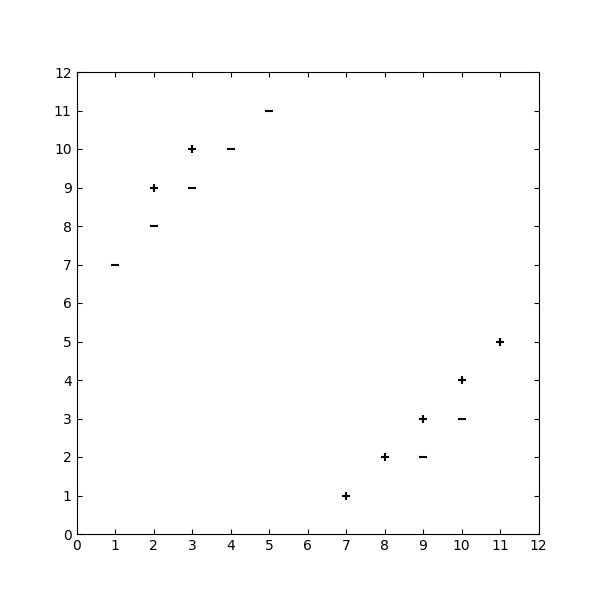
\includegraphics[width=0.6\textwidth]{images/Q2_knn.png}
				\caption{k-NN Dataset with Test Point} \label{fig:knn6_train}  % 唯一标签
			\end{figure}
			
			
			\subquestion \sall  Consider an unseen query sample $\xv^{\text{new}} = [3,11]^T$ (with horizontal coordinate 3 and vertical coordinate 11) that needs prediction, as illustrated in Figure \ref{fig:knn6_test}.
			
			\begin{figure}[H]
				\centering
				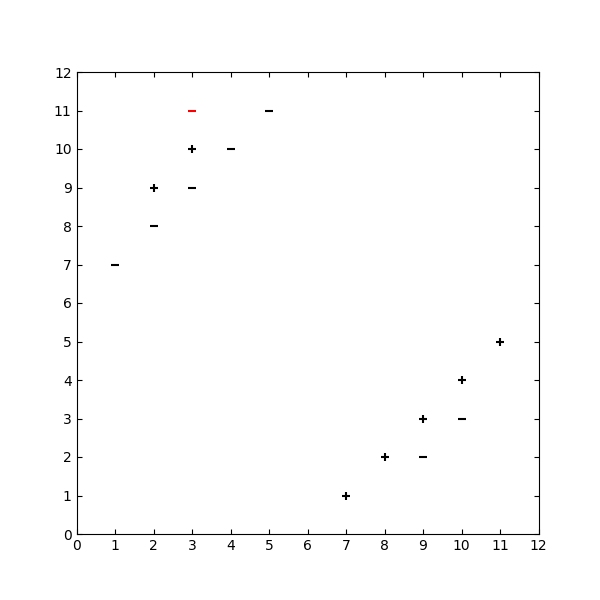
\includegraphics[width=9cm,height=9cm]{images/Q2_knn_test_point.png}
				\caption{k-NN Dataset with Test Point} \label{fig:knn6_test}  % 唯一标签
			\end{figure}
			Identify which neighborhood size(s) $k$ guarantee correct prediction for this query sample under the $k$-NN method:
			
			\begin{checkboxes}
				\checkboxchar{$\Box$} \checkedchar{$\blacksquare$}
				\choice $k = 1$
				\CorrectChoice $k = 5$
				\CorrectChoice $k = 9$
				\CorrectChoice $k = 12$
				\choice None of the above
			\end{checkboxes}
		\end{subquestions}
		
		\item[(2)] \sone Suppose you partition a large labeled dataset randomly into training and test subsets, with the goal of predicting labels for the test subset using $k$-NN. 
		
		\begin{subquestions}
			\subquestion To achieve optimal test performance, the best strategy is to select $k$ by minimizing the error rate observed on the training data. 
			
			\begin{checkboxes}
			\checkboxchar{$\Box$} \checkedchar{$\blacksquare$}
				\choice True
				\CorrectChoice False
			\end{checkboxes}
			
			\clearpage 
			
			\subquestion \sone An alternative approach divides your available training data into two parts: one for model fitting and another for validation. You then select hyperparameters that minimize validation error rather than training error. Does this validation-based selection strategy offer advantages over training-error-based selection?
			
			\begin{checkboxes}
				\checkboxchar{$\Box$} \checkedchar{$\blacksquare$}
				\CorrectChoice Yes, optimizing for validation performance is superior because minimizing training error can result in overfitting and poor generalization.
				\choice Yes, validation-based optimization ensures better test performance due to the guarantees provided by cross-validation.
				\choice No, training error minimization is preferable because validation error reduction does not improve generalization and may cause overfitting.
				\choice No, achieving the lowest possible training error is essential to guarantee optimal test set performance.
			\end{checkboxes}
			
			\subquestion \sone A colleague proposes using the test data (rather than creating a separate validation partition from the training data) for hyperparameter tuning. Would you support this proposal? Provide justification in at most 3 sentences.
			
			\begin{checkboxes}
				\checkboxchar{$\Box$} \checkedchar{$\blacksquare$}
				\choice Yes
				\CorrectChoice No
			\end{checkboxes}
			
			\begin{answer_box}[title=Your answer:,height=5cm,width=15cm]
				% 理由区域(例:No, test set should be unseen; using it for validation leads to overestimation of performance.)
				No, because using the test set for hyperparameter tuning leaks information about the test distribution into the model selection process, leading to an overestimation of final performance and undermining the fairness of the test set as truly “unseen data”.
			\end{answer_box}
		\end{subquestions}
		
		\clearpage
		
		\item[(3)] \sall You have a binary $k$-NN model with $k=4$ distinguishing between two classes: ``triangle" and ``square".
		For query point $\xv =(1,1)$, exactly two of its four closest neighbors carry label ``triangle" while the other two are labeled ``square", as displayed below. 
		
		When multiple training points have identical distances to the query, prioritize those with smaller horizontal coordinates, then by smaller vertical coordinates.
		
		\begin{figure}[H]
			\centering
			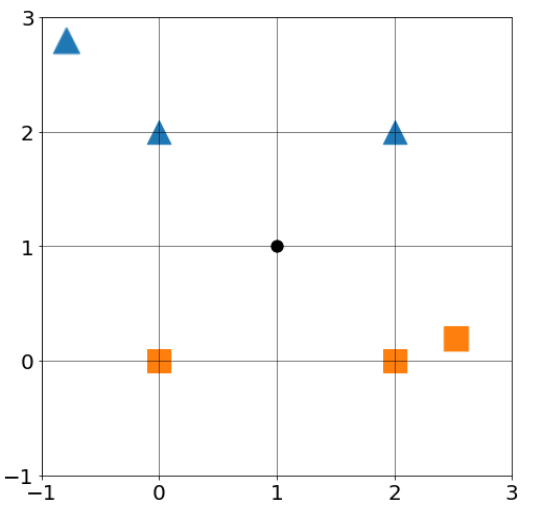
\includegraphics[width=0.5\textwidth]{images/1-1-5.png}
			\caption{k-NN Tie-Breaking} \label{fig:knn6_tie}  % 唯一标签
		\end{figure}
		
		Which modification(s) ensure that the voting procedure produces a unique class prediction for x without ties? 
		
		\begin{checkboxes}
			\checkboxchar{$\Box$} \checkedchar{$\blacksquare$}
			\choice Use $k = 2$ instead
			\CorrectChoice Flip a coin to randomly assign a label to $\xv$ (from the labels of its 4 closest points)
			\CorrectChoice Use $k = 3$ instead
			\CorrectChoice Use $k = 5$ instead
			\choice None of the above.
		\end{checkboxes}
		
		\item[(4)] \sall Evaluate the following claims regarding $k$-NN methodology and select all accurate statements:
		
		\begin{checkboxes}
			\checkboxchar{$\Box$} \checkedchar{$\blacksquare$}
			\CorrectChoice Increasing $k$ typically results in more regular and less complex decision boundaries.
			\CorrectChoice Raising the neighborhood size $k$ helps mitigate the influence of noisy observations and anomalous data points.
			\choice Setting $k$ excessively high can lead to overfitting on the training data.
			\CorrectChoice Cross-validation provides a principled approach for determining an appropriate value of $k$.
			\choice The $k$ value that achieves minimum validation error should always be avoided.
			\choice None of the above.
		\end{checkboxes}
		
		\newpage
		
		\item[(5)] The table below shows observations linking academic achievement to post-graduation income. Two predictor variables (secondary school GPA and college GPA) and one response variable (annual salary in thousands of dollars) are recorded.
		
		\begin{table}[H]
			\centering
			\begin{tabular}{cccc}
				\textbf{Student ID} & \textbf{High School GPA} & \textbf{University GPA} & \textbf{Salary} \\
				1 & 2.6 & 3.4 & 50 \\
				2 & 3.4 & 3.4 & 85 \\
				3 & 3.8 & 4.0 & 130 \\
				4 & 3.2 & 2.5 & 150 \\
				5 & 3.4 & 3.1 & 2500 \\
				6 & 3.2 & 3.1 & 70 \\
				7 & 3.8 & 3.7 & unknown \\
			\end{tabular}
			\caption{Student GPA-Salary Data} \label{tab:knn6_salary}  % 唯一标签
		\end{table}
		
		\begin{subquestions}
			\subquestion Identify which student from Students 1-6 has the smallest Euclidean distance to Student 7. Report only the Student ID.
			
			\begin{answer_box}[title=Your answer:,height=2cm,width=5cm]
				% 答案区域
				$3$
			\end{answer_box}
			
			\subquestion Your objective is to estimate Student 7's post-graduation income using $k$-NN regression, where the predicted salary equals the mean salary of the $k$ closest training samples. With $k=3$, compute your salary prediction for Student 7 in the same units as the table (thousands of dollars annually). \\
			\textbf{Round your answer to the nearest integer.}
			
			\begin{answer_box}[title=Your answer:,height=2cm,width=5cm]
				% 答案区域
				$\frac{130 + 85 + 2500}{3} = 905$
			\end{answer_box}
			
			\subquestion \sall Assume the 6 students above represent merely a sample from your complete training corpus of 10,000 students. You fit a $k$-NN regression model with Euclidean distance metric, evaluating performance via mean squared error (MSE) of salary predictions on the training data. Analyze which of the following feature transformations \textbf{could} alter the training MSE:
			
			\begin{checkboxes}
				\checkboxchar{$\Box$} \checkedchar{$\blacksquare$}
				\CorrectChoice Normalizing only ``High School GPA" as a percentage of 4.0
				\CorrectChoice Normalizing only ``University GPA" as a percentage of 4.0
				\choice Applying identical normalization (same scaling factor) to both High School GPA and University GPA
				\choice None of the above.
			\end{checkboxes}
		\end{subquestions}
		
		\clearpage
		
		\item[(6)] An archaeologist unearths a 242KB 8-inch floppy disk buried near Wean Hall containing several hundred monochrome 3×3 pixel images. Your task is to categorize each image as either a photograph ($y=+$) or artistic rendering ($y=-$) for historical analysis purposes. 
		
		You construct a $k$-NN classification system using web-sourced training images (downsampled to matching 3×3 monochrome format). Each image encodes as a $3 \times 3$ binary matrix $\xv$, with dissimilarity quantified via Hamming distance: 
		$$d(\uv, \mathbf{v}) = \sum_{i=1}^3 \sum_{j=1}^3 \mathbf{1}(\uv_{i,j} \neq \vv_{i,j}) = \text{count of differing pixels between } \uv \text{ and } \vv$$
		When selecting the $k$ closest neighbors, if multiple candidates share the same distance, expand the neighborhood to include all tied candidates in the voting. Should the final vote produce a tie, output $\hat{y}=?$. 
		Test your implementation using the samples provided below.
		
		\begin{table}[H]
			\centering
			\begin{tabular}{ccccccccccc}
				\toprule
				sample & $y$ & $x_{1,1}$ & $x_{1,2}$ & $x_{1,3}$ & $x_{2,1}$ & $x_{2,2}$ & $x_{2,3}$ & $x_{3,1}$ & $x_{3,2}$ & $x_{3,3}$  \\
				\midrule
				1 & $+$ & 0 & 0 & 1 & 0 & 1 & 1 & 0 & 0 & 0 \\
				2 & $+$ & 1 & 0 & 1 & 0 & 1 & 0 & 1 & 0 & 0 \\
				3 & $+$ & 0 & 1 & 0 & 1 & 1 & 1 & 1 & 0 & 1 \\
				4 & $-$ & 0 & 0 & 1 & 0 & 0 & 0 & 0 & 0 & 0 \\
				5 & $-$ & 1 & 0 & 1 & 1 & 1 & 0 & 0 & 1 & 1 \\
				\bottomrule
			\end{tabular}
			\caption{Training Data (Problem 6)} \label{tab:knn6_train_img}  % 唯一标签
		\end{table}
		
		\begin{table}[H]
			\centering
			\begin{tabular}{cccccccccc}
				\toprule
				sample & $x_{1,1}$ & $x_{1,2}$ & $x_{1,3}$ & $x_{2,1}$ & $x_{2,2}$ & $x_{2,3}$ & $x_{3,1}$ & $x_{3,2}$ & $x_{3,3}$  \\
				\midrule
				6 & 1 & 0 & 1 & 0 & 0 & 0 & 1 & 0 & 1 \\
				7 & 0 & 0 & 1 & 0 & 0 & 1 & 1 & 1 & 0 \\
				\bottomrule
			\end{tabular}
			\caption{Test Data (Problem 6)} \label{tab:knn6_test_img}  % 唯一标签
		\end{table}
		
		\begin{subquestions}
			\subquestion Compute the Hamming distance between samples $\xv^{(2)}$ and $\xv^{(6)}$. \\
			
			\begin{answer_box}[title=Your answer:,height=2cm,width=5cm]
				% 答案区域
				$2$
			\end{answer_box}
			
			\subquestion \sone Using $k=3$ neighbors, what class label would your $k$-NN model assign to query sample $\xv^{(7)}$?
			\begin{checkboxes}
				\checkboxchar{$\Box$} \checkedchar{$\blacksquare$}
				\CorrectChoice $\hat{y}=+$
				\choice $\hat{y}=-$
				\choice $\hat{y}=?$
			\end{checkboxes}
			
			\subquestion \sone With neighborhood size $k=5$, determine the predicted label for query sample $\xv^{(7)}$:
			\begin{checkboxes}
				\checkboxchar{$\Box$} \checkedchar{$\blacksquare$}
				\CorrectChoice $\hat{y}=+$
				\choice $\hat{y}=-$
				\choice $\hat{y}=?$
			\end{checkboxes}
			
			\subquestion \textbf{Short answer:} A colleague suggests replacing Hamming distance with Euclidean distance for potentially improved accuracy. Would this substitution likely reduce test error? Explain your reasoning. \\
			
			\begin{answer_box}[title=Your answer:, height=5cm]
				% 解释区域(例:No, pixels are binary; Euclidean distance overweights differences, Hamming is more appropriate for discrete data.)
				No, because the pixel values are binary (0 or 1), the Hamming distance and Euclidean distance produce identical neighbor rankings, so the final k-NN prediction is unaffected. Moreover, Euclidean distance requires additional square root computations, making it slightly less efficient than Hamming distance.
			\end{answer_box}
		\end{subquestions}
		
		
		\item[(7)] \textbf{Numeric answer} You possess a substantial labeled dataset for training a $k$-NN classification model. To optimize hyperparameters, you plan to conduct an exhaustive grid search over two dimensions: neighborhood size $k$ and distance function. Performance evaluation for each configuration will use cross-validation.
		
		Your grid spans 5 candidate values for $k$ (specifically: 3, 5, 7, 9, and 11) and 2 distance metrics (Euclidean and Hamming). You elect to use 10-fold cross-validation. Calculate the total number of distinct models that must be trained throughout this hyperparameter optimization procedure.
		
		\begin{answer_box}[title=Your answer:,height=2cm,width=5cm]
			% 答案区域(例:5*2*10=100)
			$5 \times 2 \times 10 = 100$
		\end{answer_box}
	\end{enumerate}
	\clearpage
	
	
	\section*{Problem 4 : Regression Tree}
	\begin{enumerate}[label=\alph*), itemsep=10pt]
		\item[(1)] You are working with the dataset shown below, where $x_1$ serves as an input variable for predicting the target $y$. Throughout this problem, each terminal node (leaf) outputs the mean $y$ value of all training samples assigned to that node, and tree construction employs the squared error (SSE) partitioning criterion.
		
		\begin{figure}[H]
			\centering
			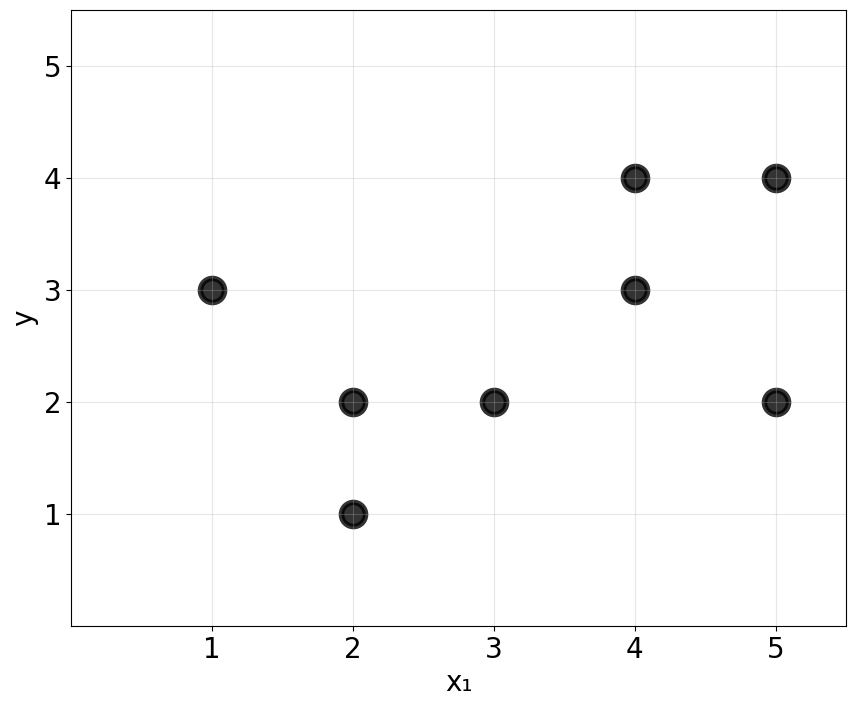
\includegraphics[width=7cm,height=6cm]{images/regression_tree_data.png}
			\caption{Regression Tree Data} \label{fig:reg5_data}  % 唯一标签
		\end{figure}
		
		\begin{subquestions}
			\subquestion Suppose you construct a regression tree with a single partition point at $x_1=4.5$ as illustrated. Determine the model's prediction for a new observation having $x_1 = 2$. Report your result with one decimal place.
			% **Could wording be better?** 
			
			\begin{figure}[H]
				\centering
				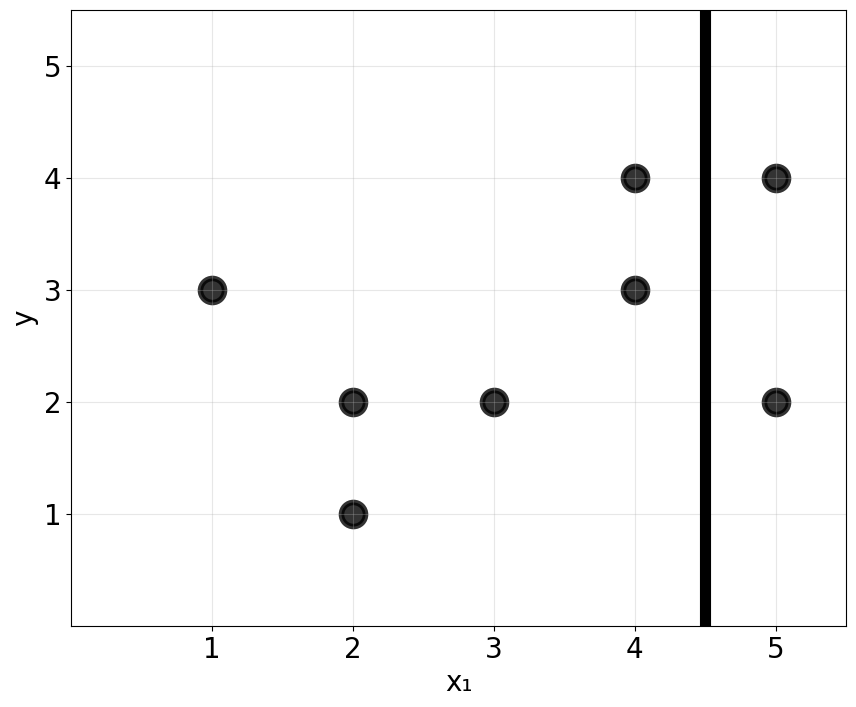
\includegraphics[width=7cm,height=6cm]{images/regression_tree_choices.png}
				\caption{Sample Regression Tree} \label{fig:reg5_sample}  % 唯一标签
			\end{figure}
			
			\begin{answer_box}[title=Your Answer,height=2cm,width=5cm]
				% 答案区域
				$y = \frac{3 + 3 + 2 + 2 + 1}{5} = 2.2$
			\end{answer_box}
			
			\clearpage
			
			\subquestion Identify which diagram below corresponds to the optimal single-split regression tree achievable for this dataset. 
			
			\begin{figure}[H]
				\centering
				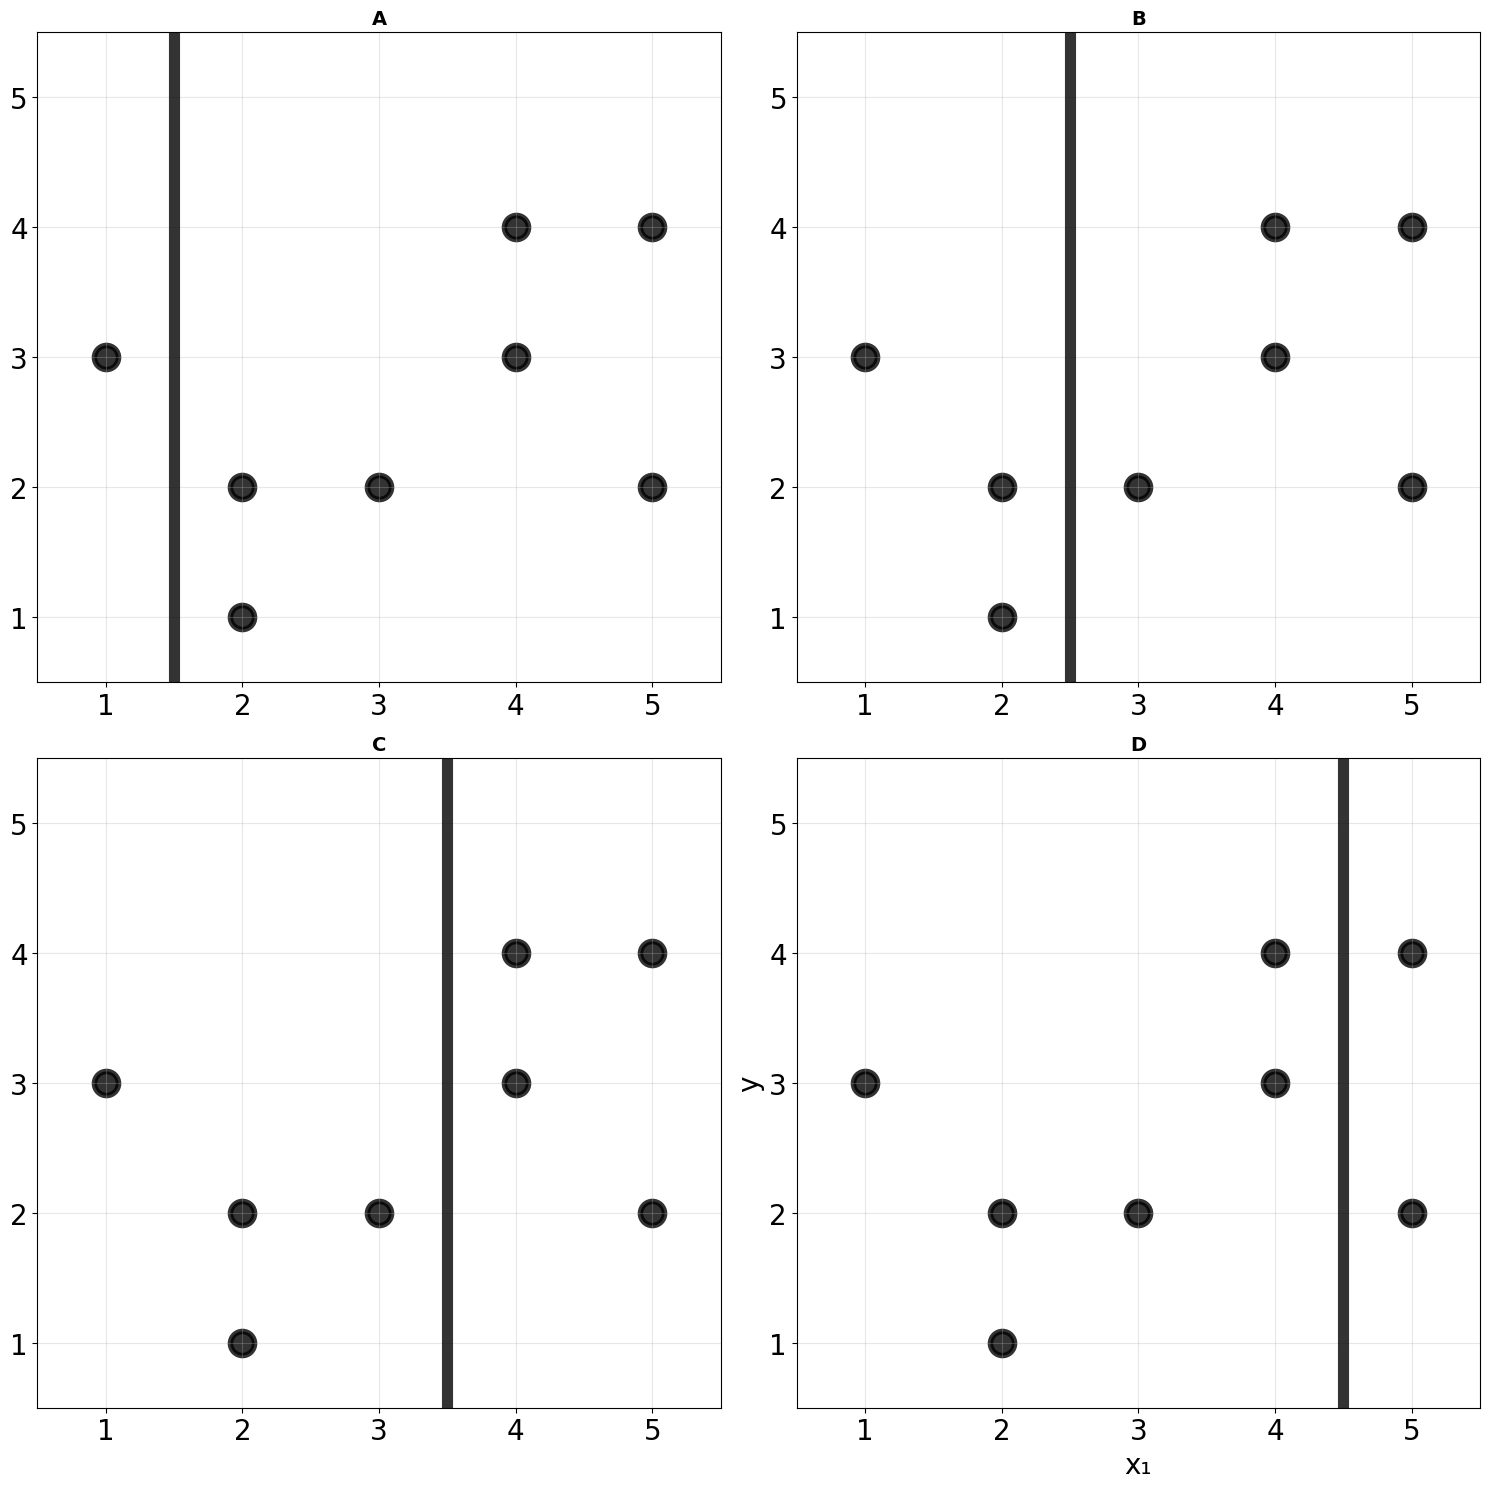
\includegraphics[width=15cm,height=15cm]{images/regression_tree_one.png}
				\caption{Answer Choices} \label{fig:reg5_depth1}  % 唯一标签
			\end{figure}
			
			\begin{checkboxes}
				\checkboxchar{$\Box$} \checkedchar{$\blacksquare$}
				\choice A 
				\choice B 
				\CorrectChoice C 
				\choice D 
			\end{checkboxes}
			
			\clearpage
			
			\subquestion Consider extending the tree from the previous question by adding one additional \textbf{level} using the same partitioning criterion. Select the resulting tree structure: 
			
			\begin{figure}[H]
				\centering
				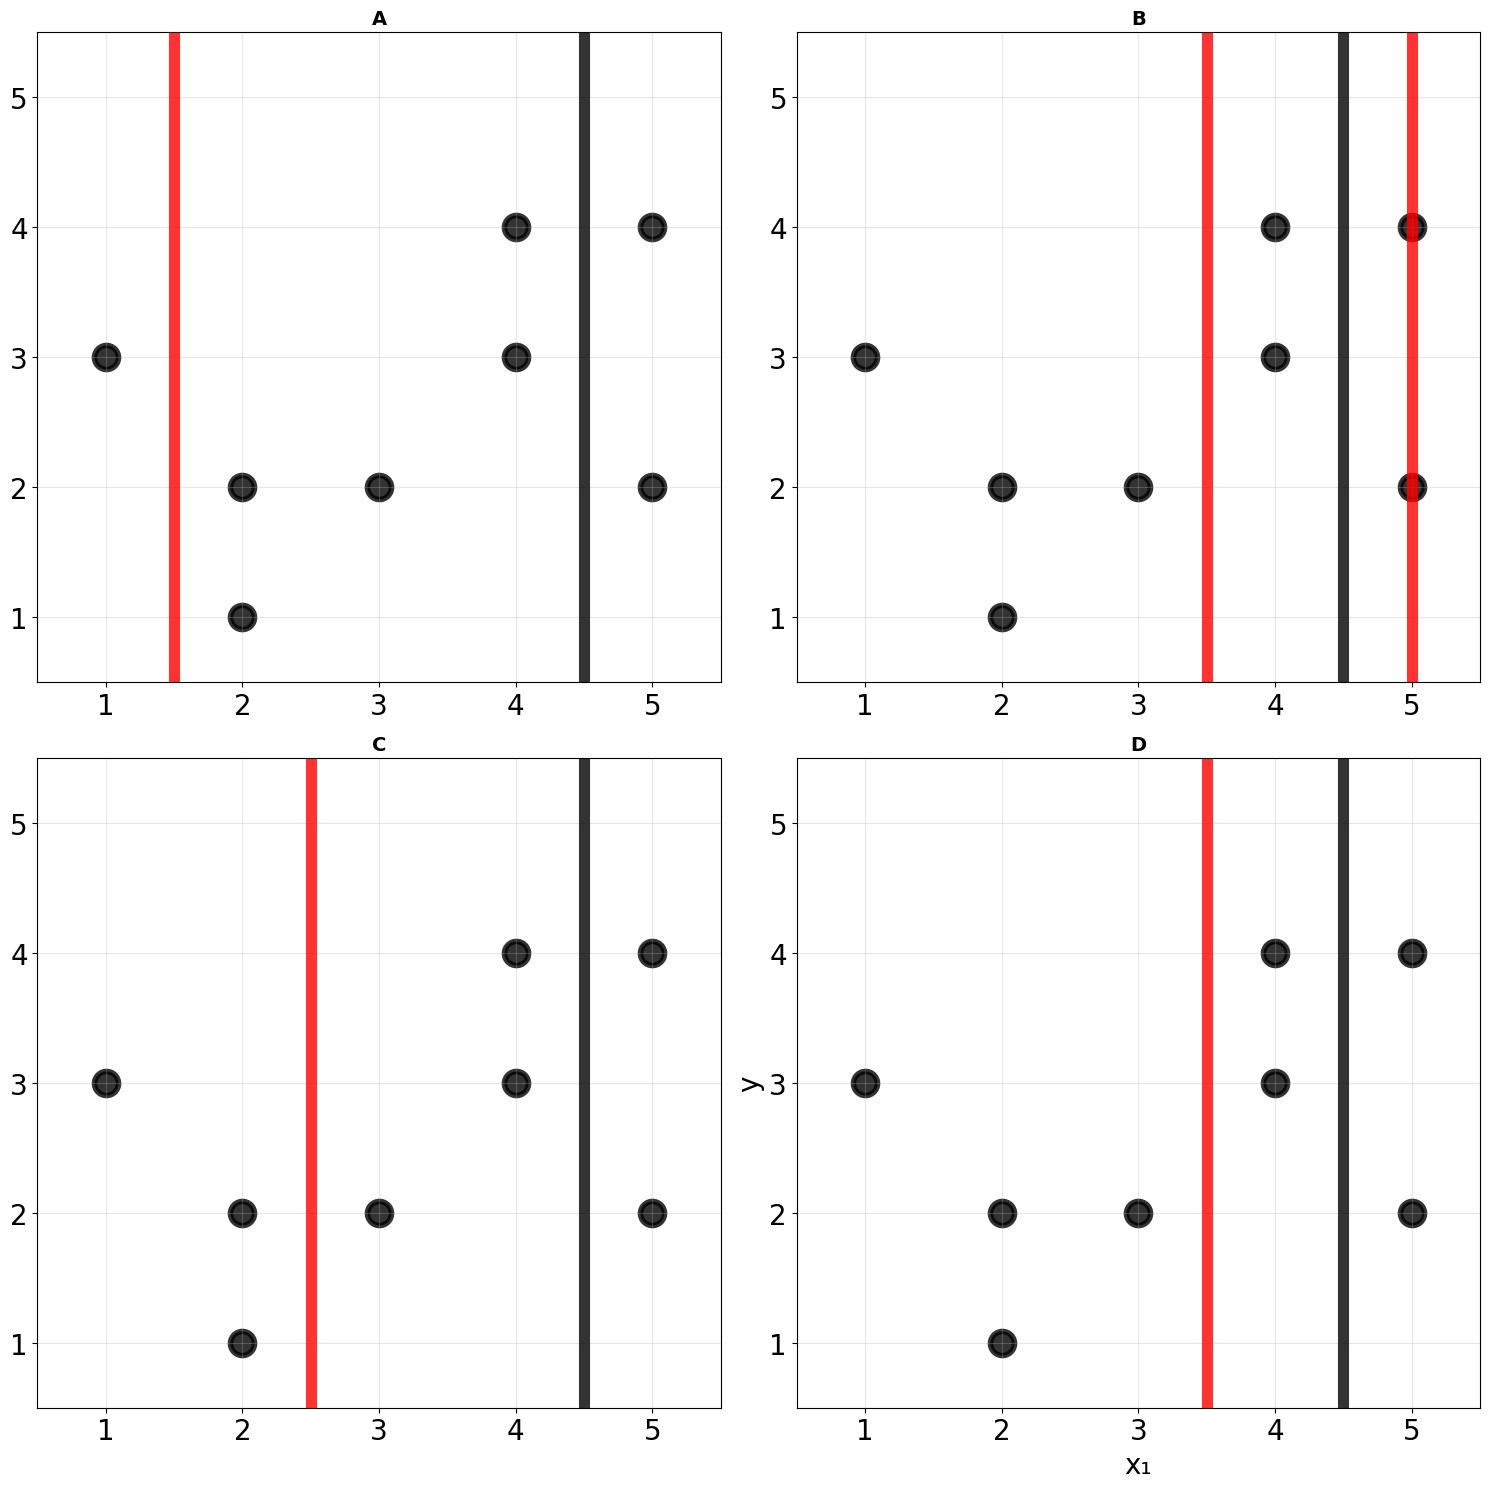
\includegraphics[width=12cm,height=12cm]{images/regression_tree_two_levels.png}
				\caption{Answer Choices} \label{fig:reg5_depth2}  % 唯一标签
			\end{figure}
			
			\begin{checkboxes}
				\checkboxchar{$\Box$} \checkedchar{$\blacksquare$}
				\choice A
				\choice B
				\choice C
				\CorrectChoice D
			\end{checkboxes}
		\end{subquestions}
		
		\item[(2)] Given an arbitrary dataset, suppose you construct a depth-2 regression tree by selecting optimal partitions at each decision node sequentially. Does this greedy construction procedure necessarily yield the depth-2 tree with minimum achievable training error? (\textbf{Hint:} Reflect on the algorithmic nature of regression tree learning)
		
		\begin{answer_box}[title=Your answer:,height=5cm]
			% 解释区域
			No, because the greedy algorithm makes locally optimal choices at each node without considering the global structure of the tree. This can lead to suboptimal splits that do not minimize overall training error for the entire depth-2 tree.
		\end{answer_box}
	\end{enumerate}	
	
	\section*{Problem 5: Decision Tree }
	
	We examine decision tree construction principles using the training data below. Dataset \(D\) comprises 8 observations, each characterized by three features \((A, B, C)\) and a target variable \(Y\).
	
	\begin{center}
		\begin{tabular}{|c|c|c|c|}
			\hline
			\(A\) & \(B\) & \(C\) & \(Y\) \\ 
			\hline
			1 & 2 & 0 & 1     \\ 
			\hline
			0 & 1 & 0 & 0     \\ 
			\hline
			0 & 0 & 1 & 0     \\ 
			\hline
			0 & 2 & 0 & 1     \\ 
			\hline
			1 & 1 & 0 & 1     \\ 
			\hline
			1 & 0 & 1 & 0     \\ 
			\hline
			1 & 2 & 1 & 0     \\ 
			\hline
			1 & 1 & 0 & 1     \\ 
			\hline
		\end{tabular}
	\end{center}
	
	Apply the dataset above to respond to the subsequent questions.  
	
	Important specifications:
	\begin{itemize}[leftmargin=*]
		\item \emph{Perform all intermediate computations without rounding!} Report your final rounded answers in the designated answer boxes.
		\item Unless stated otherwise, provide numerical results with 4-digit precision (e.g. 0.1234).
		\item Throughout this problem, we adopt the convention that terminal nodes (leaves) are excluded from node counts, and therefore do not contribute to depth or split tallies. (For instance, a tree with a single decision node has depth 1 and contains 1 split.)
		\item The dataset includes repeated observations; treat each row as a distinct sample without removing duplicates.
	\end{itemize}
	
	\textit{Note}: Demonstrating your computational steps is optional but encouraged to facilitate partial credit. Only the numerical value in the left box receives grading.
	
	
	% 问题1:计算Y的熵H(Y)
	\begin{questions}
		\item[(1)] Compute the Shannon entropy \(H(Y)\) for the target variable \(Y\), expressed in bits. For this and all following questions, reporting values in \emph{bits} requires using \(\log\) base 2 in your computations.\footnote{Alternative logarithm bases yield different units: base \(e\) produces \emph{nats}, while base 10 yields \emph{bats}.} (Report a single value rounded to four decimal places, e.g. 0.1234)
		
		\begin{minipage}[t]{0.25\textwidth}
			\begin{answer_box}[title=$H(Y)$]
				% 在此处填写答案
				1 bit
			\end{answer_box}
		\end{minipage}
		\begin{minipage}[t]{0.7\textwidth}
			\begin{answer_box}[title=Work]
				% 在此处展示计算过程
				$P(Y = 0) = 4/8 = 0.5;$ \\
				$P(Y = 1) = 4/8 = 0.5;$ \\
				$H(Y) = -\sum P(Y) \log_2 P(Y) = -[0.5 \log_2 0.5 + 0.5 \log_2 0.5] = 1$ bit.
			\end{answer_box}
		\end{minipage}
		
		
		% 问题2:计算Y与A的互信息I(Y;A)
		\item[(2)] Calculate the mutual information \(I(Y; A)\) between target \(Y\) and feature \(A\), measured in bits. (Provide a single number rounded to four decimal places, e.g. 0.1234)
		
		\begin{minipage}[t]{0.25\textwidth}
			\begin{answer_box}[title=$I(Y;A)$,height=6cm]
				% 在此处填写答案
				0.0488 bits
			\end{answer_box}
		\end{minipage}
		\begin{minipage}[t]{0.7\textwidth}
			\begin{answer_box}[title=Work,height=6cm]
				% 在此处展示计算过程
				$P(Y=0|A=1)=\frac25;$\\
				$P(Y=1|A=1)=\frac35=0.6;$\\
				$H(Y|A=1)=-\sum P(Y|A) \log_2 P(Y|A) = -[\frac25 \log_2 \frac25 + \frac35 \log_2 \frac35];$ \\
				$P(Y=0|A=0)=\frac23;$\\
				$P(Y=1|A=0)=\frac13;$\\
				$H(Y|A=0)=-\sum P(Y|A) \log_2 P(Y|A) = -[\frac23 \log_2 \frac23 + \frac13 \log_2 \frac13];$\\
				$P(A=1)=\frac58;$\\
				$P(A=0)=\frac38;$\\
				$H(Y|A)=P(A=1)H(Y|A=1)+P(A=0)H(Y|A=0)=\frac58 H(Y|A=1)+\frac38 H(Y|A=0)$;\\
				$I(Y;A) = H(Y) - H(Y|A) \approx 0.0488$ bits. \\
			\end{answer_box}
		\end{minipage}
		
		
		% 问题3:计算Y与B的互信息I(Y;B)
		\item[(3)] Determine the mutual information \(I(Y; B)\) between target \(Y\) and feature \(B\), in bits. (Provide a single number rounded to four decimal places, e.g. 0.1234)
		
		\begin{minipage}[t]{0.25\textwidth}
			\begin{answer_box}[title=$I(Y;B)$,height=10cm]
				% 在此处填写答案
				0.3113 bits
			\end{answer_box}
		\end{minipage}
		\begin{minipage}[t]{0.7\textwidth}
			\begin{answer_box}[title=Work,height=10cm]
				% 在此处展示计算过程
				$P(Y=0|B=0)=1;$\\
				$H(Y|B=0)=-\sum P(Y|B) \log_2 P(Y|B) = -[1\log_2 1]=0;$\\
				$P(Y=0|B=1)=\frac13;$\\
				$P(Y=1|B=1)=\frac23;$\\
				$H(Y|B=1)=-\sum P(Y|B) \log_2 P(Y|B) = -[\frac13 \log_2 \frac13 + \frac23 \log_2 \frac23];$\\
				$P(Y=0|B=2)=\frac13;$\\
				$P(Y=1|B=2)=\frac23;$\\
				$H(Y|B=2)=-\sum P(Y|B) \log_2 P(Y|B) = -[\frac13 \log_2 \frac13 + \frac23 \log_2 \frac23];$\\
				$P(B=0)=\frac28=\frac14;$\\
				$P(B=1)=\frac38;$\\
				$P(B=2)=\frac38;$\\
				$H(Y|B)=P(B=0)H(Y|B=0)+P(B=1)H(Y|B=1)+P(B=2)H(Y|B=2)=\frac14 \cdot 0 + \frac38 H(Y|B=1) + \frac38 H(Y|B=2)$;\\
				$I(Y;B) = H(Y) - H(Y|B) \approx 0.3113$ bits. \\
			\end{answer_box}
		\end{minipage}
		
		
		% 问题4:计算Y与C的互信息I(Y;C)
		\item[(4)] Evaluate the mutual information \(I(Y; C)\) between target \(Y\) and feature \(C\), measured in bits. (Report a single number rounded to four decimal places, e.g. 0.1234)
		
		\begin{minipage}[t]{0.25\textwidth}
			\begin{answer_box}[title=$I(Y;C)$,height=6cm]
				% 在此处填写答案
				0.5488 bits
			\end{answer_box}
		\end{minipage}
		\begin{minipage}[t]{0.7\textwidth}
			\begin{answer_box}[title=Work,height=6cm]
				% 在此处展示计算过程
				$P(Y=0|C=0)=\frac15;$\\
				$P(Y=1|C=0)=\frac45;$\\
				$H(Y|C=0)=-\sum P(Y|C) \log_2 P(Y|C) = -[\frac15 \log_2 \frac15 + \frac45 \log_2 \frac45];$\\
				$P(Y=0|C=1)=1;$\\
				$H(Y|C=1)=-\sum P(Y|C) \log_2 P(Y|C) = -[1\log_2 1]=0;$\\
				$P(C=0)=\frac58;$\\
				$P(C=1)=\frac38;$\\
				$H(Y|C)=P(C=0)H(Y|C=0)+P(C=1)H(Y|C=1)=\frac58 H(Y|C=0)+\frac38 \cdot 0$;\\
				$I(Y;C) = H(Y) - H(Y|C) \approx 0.5488$ bits. \\
			\end{answer_box}
		\end{minipage}
		
		
		% 问题5:选择第一个分裂属性
		\item[(5)] Select one: Using the dataset provided, identify which feature ($A$, $B$, or $C$) would be selected for the root split by a decision tree learner employing mutual information as its selection criterion.
		
		\begin{checkboxes}
			\checkboxchar{$\Box$} \checkedchar{$\blacksquare$}
			\choice $A$
			\choice $B$
			\CorrectChoice $C$
		\end{checkboxes}
		
		
		% 问题6:选择第二个分裂属性
		\item[(6)] Select one: Following the initial partition, which feature would the tree learning algorithm choose for the subsequent split, assuming mutual information guides feature selection? (\emph{Hint:} Observe that this question presumes \emph{exactly one} feature will be selected second.)
		
		\begin{checkboxes}
			\checkboxchar{$\Box$} \checkedchar{$\blacksquare$}
			\choice $A$
			\CorrectChoice $B$
			\choice $C$
		\end{checkboxes}
		
		
		% 问题7:计算树的深度
		\item[(7)] Suppose the learning procedure continues recursively until achieving perfect classification accuracy on the training data. Report the resulting tree's depth.
		
		\begin{minipage}[t]{0.25\textwidth}
			\begin{answer_box}[title=Depth]
				% 在此处填写答案
				$2$
			\end{answer_box}
		\end{minipage}
		
		
		% 问题8:绘制决策树
		\item[(8)] Construct and illustrate the complete decision tree learned from the dataset above, utilizing mutual information for split selection and growing until zero training error is achieved. Mark each internal (non-terminal) node with its splitting feature (e.g. $B$), annotate edges with the corresponding feature values (e.g. 1 or 0), and label terminal nodes with their predicted class (e.g. $Y=0$). You may insert an image file using the provided commented \LaTeX{} code, substituting your filename for \textit{DecTree.png}. Hand-drawn diagrams are acceptable. For programmatic visualization, you may optionally use libraries such as \texttt{matplotlib} or \texttt{graphviz}.
		
		\begin{answer_box}[title=Decision Tree, height=9cm]
			% 插入图片示例(取消注释并替换文件名即可)
			\begin{center}
			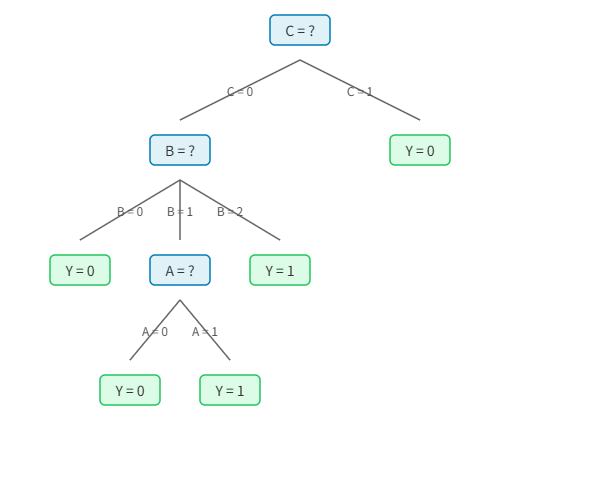
\includegraphics[width=0.8\linewidth]{DecTree.png}
			\end{center}
		\end{answer_box}
		
		
		% 问题9:预测标签
		\item[(9)] Apply your learned decision tree to classify the test instances listed below. The table displays the feature values for reference. Record the predictions for all samples sequentially, delimited by commas. For instance, if your predictions are 1,0,1,0, format as: 1,0,1,0
		
		\begin{center}
			\begin{tabular}{|c|c|c|}
				\hline
				$A$ & $B$ & $C$ \\ 
				\hline
				1 & 1 & 0 \\ 
				\hline
				1 & 2 & 0 \\ 
				\hline
				0 & 1 & 0 \\ 
				\hline
				0 & 2 & 0 \\ 
				\hline
				0 & 1 & 1 \\ 
				\hline
				1 & 1 & 1 \\ 
				\hline
			\end{tabular}
		\end{center}
		
		\begin{answer_box}[title=Predicted Labels]
			% 在此处填写预测结果(例:1,0,1,0,0,1)
			1,1,0,1,0,0
		\end{answer_box}
		
	\end{questions}
	
	
	
	\section*{Problem 6 : Logistic Regression}
	\label{sec:warm-up}
	
	\begin{enumerate}
		\item[(1)] Complete the following analytical exercises prior to beginning the implementation portion of this assignment.
		
		You are provided with a training set containing 4 observations. For each sample $i \in \{1, 2, 3, 4\}$, the notation $x_k^{(i)}$ represents the value of the $k$-th feature ($k \in \{1, 2, 3\}$) in feature vector $\xv^{(i)}$, while $y^{(i)}$ denotes the corresponding binary class label.
		
		\begin{center}
			\begin{tabular}{|c|c|c|c|c|c|c|}
				\hline
				$i$ & $x_{1}$ & $x_{2}$ & $x_{3}$ & $y$ \\ \hline
				1   & 0       &       0 &       1 & 0   \\ \hline
				2   & 0       &       1 &       0 & 1   \\ \hline
				3   & 0       &       1 &       1 & 1   \\ \hline
				4   & 1       &       0 &       0 & 0   \\ \hline
				
			\end{tabular}
		\end{center}
		
		A binary classification model using logistic regression has been fitted to this data, yielding the learned weight vector:
		
		\[\thetav = \begin{bmatrix}1.5 & 2 & 1\end{bmatrix}^T.\]
		
		\textit{Note}: This model excludes the \textbf{bias term} (operates without an intercept).
		
		Employ the dataset above to address the subsequent questions. Report all numerical results as single values rounded to four decimal places (format: 0.1234). Presenting your derivations is optional but encouraged for partial credit consideration.
		
		\begin{enumerate}[label=\alph*), itemsep=10pt]
			\item[(a)] Evaluate $J(\thetav)$, defined as $\frac{1}{N}$ multiplied by the negative log-likelihood computed across the provided data using parameter vector $\thetav$. (Apply natural logarithm with base $e$ throughout).
			
			\begin{your_solution}[title=$J(\thetav)$,height=2cm,width=3cm]
				% YOUR ANSWER 
				$0.7975$
			\end{your_solution}
			
			\begin{your_solution}[title=Work,height=6cm]
				% YOUR ANSWER
				$J(\thetav) = -\frac{1}{N} \sum_{i=1}^{N} \left[ y^{(i)} \log(\sigma(\thetav^T x^{(i)})) + (1 - y^{(i)}) \log(1 - \sigma(\thetav^T x^{(i)})) \right]$\\
				$=\frac{1}{N}\sum_{i=1}^N-y^{(i)}(\thetav^T \xv^{(i)})+\log(1+\exp(\thetav^T \xv^{(i)}))$\\
				$=\frac14\left[(-0+\log(1+e^1))+(-2+\log(1+e^2))+(-3+\log(1+e^3))+(-0+\log(1+e^{1.5}))\right]$\\
				$\approx 0.7975$
			\end{your_solution}
			
			\pagebreak
			
			\item[(b)] Compute the partial derivatives $\frac{\partial J(\thetav)}{\partial \theta_j}$ for each weight component $\theta_{j}$ where $j \in \{1, 2, 3\}$.
			
			\begin{your_solution}[title=$\partial J(\thetav)/\partial \theta_1$,height=1.8cm,width=5.2cm]
				% YOUR ANSWER 
				$0.2044$
			\end{your_solution}
			\begin{your_solution}[title=$\partial J(\thetav)/\partial \theta_2$,height=1.8cm,width=5.2cm]
				% YOUR ANSWER 
				$-0.0417$
			\end{your_solution}
			\begin{your_solution}[title=$\partial J(\thetav)/\partial \theta_3$,height=1.8cm,width=5.2cm]
				% YOUR ANSWER 
				$0.1709$
			\end{your_solution}
			
			\begin{your_solution}[title=Work,height=18cm]
				% YOUR ANSWER
				$\frac{\partial J}{\partial\theta_j}=\frac{1}{N}\sum_{i=1}^N(\sigma(\thetav^Tx^{(i)})-y^{(i)})x_j^{(i)}$\\
				where $\sigma(z)=\frac{1}{1+\exp(-z)}$\\
				For $\theta_1$: \\
				$\frac{\partial J}{\partial \theta_1} = \frac{1}{4}[(\sigma(1.5\times0+2\times0+1\times1)-0)\times0 + (\sigma(1.5\times0+2\times1+1\times0)-1)\times0 + (\sigma(1.5\times0+2\times1+1\times1)-1)\times0 + (\sigma(1.5\times1+2\times0+1\times0)-0)\times1]$\\
				$= \frac{1}{4}[0 + 0 + 0 + \sigma(1.5)] \approx 0.2044$\\
				For $\theta_2$: \\
				$\frac{\partial J}{\partial \theta_2} = \frac{1}{4}[(\sigma(1.5\times0+2\times0+1\times1)-0)\times0 + (\sigma(1.5\times0+2\times1+1\times0)-1)\times1 + (\sigma(1.5\times0+2\times1+1\times1)-1)\times1 + (\sigma(1.5\times1+2\times0+1\times0)-0)\times0]$\\
				$= \frac{1}{4}[0 + (\sigma(2)-1) + (\sigma(3)-1) + 0] \approx -0.0417$\\
				For $\theta_3$: \\
				$\frac{\partial J}{\partial \theta_3} = \frac{1}{4}[(\sigma(1.5\times0+2\times0+1\times1)-0)\times1 + (\sigma(1.5\times0+2\times1+1\times0)-1)\times0 + (\sigma(1.5\times0+2\times1+1\times1)-1)\times1 + (\sigma(1.5\times1+2\times0+1\times0)-0)\times0]$\\
				$= \frac{1}{4}[(\sigma(1)-0)\times1 + (\sigma(3)-1) + 0] \approx 0.1709$\\	
			\end{your_solution}
			
			
			\clearpage
			
			\item[(c)] Apply the gradient descent update rule $\theta_j \leftarrow \theta_j - \eta \frac{\partial J(\thetav)}{\partial \theta_j}$ to revise each parameter, then report the resulting numerical values of the updated weight vector $\thetav$. Set step size $\eta = 1$.
			
			\begin{your_solution}[title=$\theta_1$,height=1.8cm,width=5.2cm]
				% YOUR ANSWER 
				$1.2956$
			\end{your_solution}
			\begin{your_solution}[title=$\theta_2$,height=1.8cm,width=5.2cm]
				% YOUR ANSWER 
				$2.0417$
			\end{your_solution}
			\begin{your_solution}[title=$\theta_3$,height=1.8cm,width=5.2cm]
				% YOUR ANSWER 
				$0.8291$
			\end{your_solution}
			
			\begin{your_solution}[title=Work, height=6cm]
				% YOUR ANSWER 
				$\theta_1 \leftarrow 1.5 - 1 \times 0.2044 \approx 1.2956$\\
				$\theta_2 \leftarrow 2 - 1 \times (-0.0417) \approx 2.0417$\\
				$\theta_3 \leftarrow 1 - 1 \times 0.1709 \approx 0.8291$\\
			\end{your_solution}
			
			
		\end{enumerate}
		
		\item[(2)] 
		
		\begin{enumerate}[label=\alph*), itemsep=10pt]
			\item[(a)] \sall Identify all valid statements regarding logistic regression:
			
			{%
				\checkboxchar{$\Box$} \checkedchar{$\blacksquare$}
				\begin{checkboxes}
					\checkboxchar{$\Box$} \checkedchar{$\blacksquare$}
					\CorrectChoice The binary logistic regression framework accommodates both real-valued and discrete binary input features.
					\CorrectChoice Without feature transformations, binary logistic regression produces a linear separating hyperplane in the feature space.
					\choice The logistic sigmoid activation function exhibits convex geometry.
					\choice None of the above.
				\end{checkboxes}
			}
			
			
			
			
			\item[(b)] \sall Recognizing that the negative log-likelihood objective is convex, select all accurate claims about optimizing logistic regression via mini-batch stochastic gradient descent:
			
			{%
				\checkboxchar{$\Box$} \checkedchar{$\blacksquare$}
				\begin{checkboxes}
					\checkboxchar{$\Box$} \checkedchar{$\blacksquare$}
					\choice The optimization procedure may become trapped at suboptimal local minima when applied to small-scale datasets.
					\choice Convergence to the global optimum is guaranteed irrespective of the chosen step size.
					\choice The optimization procedure may become trapped at suboptimal local minima when applied to large-scale datasets.
					\choice Convergence to the global optimum is guaranteed irrespective of the chosen batch size.
					\CorrectChoice None of the above.
				\end{checkboxes}
			}
			
			
			
			\vspace*{1.2cm}
			
			\item[(c)] \sone For binary logistic regression, the \emph{mean} negative log-likelihood $J(\thetav)$ admits the representation
			$$J(\thetav) = \frac{1}{N}\sum_{i=1}^N  \left[-y^{(i)}\left(\thetav^T \xv^{\left(i\right)}\right)+\log\left(1+\exp(\thetav^T \xv^{\left(i\right)})\right)\right]$$
			where $\xv^{(i)}\in \mathbb{R}^{M+1}$ denotes the feature vector for sample $i$, $y^{(i)}\in\{0, 1\}$ represents the binary label for sample $i$, and $\thetav\in\mathbb{R}^{M+1}$ is the parameter vector. To implement ridge-regularized logistic regression (incorporating $\ell_2$ penalty), we augment the objective as follows:
			$$ f(\thetav) = J(\thetav) + \lambda \frac{1}{2}\sum_{j=0}^M \theta_j^2$$
			where $\lambda$ controls regularization strength and $\theta_j$ denotes the $j$-th component of $\thetav$. When performing gradient-based optimization with step size $\eta$ to update parameter $\theta_k$, identify the correct update formula:
			
			\begin{checkboxes}
				% YOUR ANSWER
				\checkboxchar{$\Box$} \checkedchar{$\blacksquare$}
				\choice 
				$\theta_k\leftarrow \theta_k + \eta \frac{\partial f(\thetav)}{\partial \theta_k}$ where 
				$ \frac{\partial f(\thetav)}{\partial \theta_k}=\frac{1}{N}\sum_{i=1}^N \left[x^{(i)}_k\left(y^{(i)} -\frac{\exp(\thetav^T \xv^{(i)})}{1+\exp(\thetav^T \xv^{(i)})} \right)\right]+\lambda \theta_k$
				\choice 
				$\theta_k\leftarrow \theta_k + \eta \frac{\partial f(\thetav)}{\partial \theta_k}$ where 
				$ \frac{\partial f(\thetav)}{\partial \theta_k}=\frac{1}{N}\sum_{i=1}^N \left[x^{(i)}_k\left(-y^{(i)} +\frac{\exp(\thetav^T \xv^{(i)})}{1+\exp(\thetav^T \xv^{(i)})} \right)\right]-\lambda \theta_k$
				\CorrectChoice
				$\theta_k\leftarrow \theta_k - \eta \frac{\partial f(\thetav)}{\partial \theta_k}$ where 
				$ \frac{\partial f(\thetav)}{\partial \theta_k}=\frac{1}{N}\sum_{i=1}^N \left[x^{(i)}_k\left(-y^{(i)} +\frac{\exp(\thetav^T \xv^{(i)})}{1+\exp(\thetav^T \xv^{(i)})} \right)\right]+\lambda \theta_k$
				\choice
				$\theta_k\leftarrow \theta_k - \eta \frac{\partial f(\thetav)}{\partial \theta_k}$ where 
				$ \frac{\partial f(\thetav)}{\partial \theta_k}=\frac{1}{N}\sum_{i=1}^N \left[x^{(i)}_k\left(-y^{(i)} -\frac{\exp(\thetav^T \xv^{(i)})}{1+\exp(\thetav^T \xv^{(i)})} \right)\right]+\lambda \theta_k$
			\end{checkboxes}
			
			\vspace*{1.2cm}
			
			\item[(d)] Consider fitting a logistic regression classifier to training data $\mathcal{D}_{train}$ comprising $M$ input features and binary outputs $\yv \in \{0, 1\}$. The third predictor, $\xv_3$, perfectly partitions the training samples. Specifically, all instances satisfying $\xv_3 \geq 1$ belong to class $y=1$, while the feature $\xv_3$ takes values uniformly distributed over the interval [0, 2].
			
			\begin{enumerate}[label=(\roman*), leftmargin=*]
				
				\item \sone
				The plots below illustrate how the predicted probability $\hat{P}(y=1)$ varies as a function of $\xv_3$. After extensive training via SGD (numerous epochs, $>>100$), which plot most accurately characterizes your model's behavior? \textbf{Justify your selection}.
				
				\begin{figure}[h]
					\centering
					% First figure
					\begin{subfigure}[t]{0.42\textwidth}
						\centering
						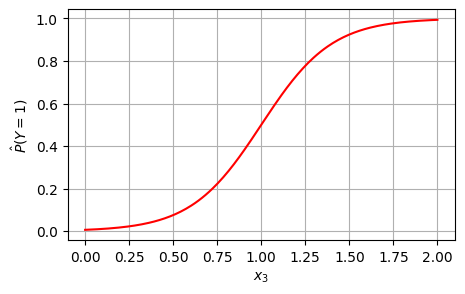
\includegraphics[width=\textwidth]{fig/Plot A.png}
						\caption{}
					\end{subfigure}
					\hfill
					% Second figure
					\begin{subfigure}[t]{0.42\textwidth}
						\centering
						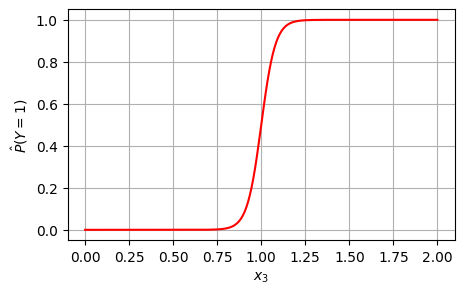
\includegraphics[width=\textwidth]{fig/Plot B.png}
						\caption{}
					\end{subfigure}
				\end{figure}
				
				\textit{Hint}: Imagine discovering a weight configuration that achieves complete linear separation of the data. Consider the implied probabilities for each sample and whether further weight adjustments could enhance the likelihood. What trajectory would the coefficient for $\xv_j$ follow?
				
				\begin{your_solution}[height=5cm]
					% YOUR ANSWER 
					Choice (b) is correct. \\
					Since feature $\xv_3$ perfectly separates the classes, logistic regression will attempt to push the decision boundary towards infinity to maximize the likelihood. As a result, the predicted probabilities will approach 0 for $\xv_3 < 1$ and 1 for $\xv_3 \geq 1$, leading to a step function-like behavior as shown in plot (b). Plot (a) would imply that the model is not fully utilizing the perfect separation provided by $\xv_3$.
				\end{your_solution}
				
				\item \sone   
				Following model training, you evaluate performance on a held-out validation set $\mathcal{D}_{validation}$, producing the visualization shown below.
				
				\begin{center}
					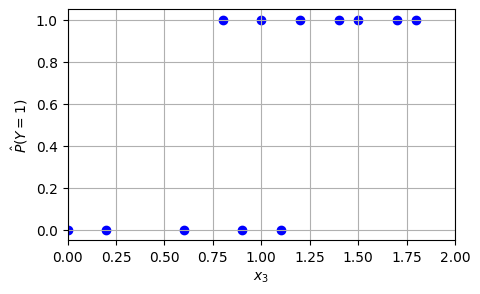
\includegraphics[width=6cm]{fig/Plot Validation.png}
				\end{center}
				
				A colleague named Neural reviews your results and recommends incorporating L2 regularization into your training objective. 
				
				\sone What effect would regularization have on the learned parameter values?
				
				
				{%
					
					\begin{checkboxes}
						\checkboxchar{$\Box$} \checkedchar{$\blacksquare$}
						\choice $\ell_2$ regularization constrains parameter growth by normalizing the weight vector to unit norm.
						\choice $\ell_2$ regularization prevents parameter divergence by setting certain weights exactly to zero, effectively performing feature elimination. 
						\CorrectChoice $\ell_2$ regularization controls parameter magnitude by shrinking weight values toward (but not necessarily to) zero, diminishing feature influence without complete removal. 
						\choice None of the above.
					\end{checkboxes}
				}
				
				
			\end{enumerate}
		\end{enumerate}
		
	\end{enumerate}
	\section*{Problem 7 : PCA}
	
	\begin{enumerate}
		\item[(1)] Consider a binary classification scenario with observations residing in two-dimensional space, partitioned into two classes:  
		\[
		c_{1}=\left\{ \begin{bmatrix} 2 \\ 1 \end{bmatrix}, \begin{bmatrix} 2 \\ 2 \end{bmatrix}, \begin{bmatrix} 2 \\ 3 \end{bmatrix} \right\}, \quad c_{2}=\left\{ \begin{bmatrix} 4 \\ 3 \end{bmatrix}, \begin{bmatrix} 5 \\ 3 \end{bmatrix}, \begin{bmatrix} 6 \\ 4 \end{bmatrix} \right\}
		\]
		
		For this problem, although you are allowed to use Python for aiding computations, you are required to show all intermediate steps. You may use \texttt{numpy} for matrix operations (e.g., \texttt{numpy.linalg.eig}, \texttt{numpy.cov}) and \texttt{matplotlib.pyplot} for visualization.
		
		
		\subsubsection*{Apply global PCA to identify the optimal projection direction for this dataset.}
		\begin{enumerate}
			\item[(a)] Derive the linear equation characterizing this principal direction through the data centroid, formatted as $\mathbf{w}^{T} \mathbf{x} + w_{0} = 0$, where 
			\[
			\mathbf{x} = \begin{bmatrix} x_{1} \\ x_{2} \end{bmatrix} \quad \text{and} \quad \mathbf{w} = \begin{bmatrix} w_{1} \\ w_{2} \end{bmatrix}
			\]
			with $w_{0}$ representing the offset parameter. Visualize this hyperplane $\mathbf{w}^{T} \mathbf{x} + w_{0} = 0$ together with all data points and the direction vector $\mathbf{w}$ originating from the centroid.

			\item[(b)] Transform all observations onto the principal component axis, then reconstruct them back to the original space. Visualize the resulting reconstructed coordinates.
			
			\item[(c)] Calculate the aggregate mean squared error (MSE) quantifying reconstruction loss across all samples (measuring discrepancy between original and reconstructed coordinates).
			
			\item[(d)] Compute the Fisher discriminant ratio for this projection, formulated as 
			\[
			FR = \frac{(m_{1} - m_{2})^{2}}{\sigma_{1}^{2} + \sigma_{2}^{2}},
			\]
			where $m_{i}$ represents the centroid of class $i$ samples after projection, and $\sigma_{i}^{2}$ denotes the corresponding variance. Evaluate $FR$ using the one-dimensional projected coordinates (not the two-dimensional reconstructions).
		\end{enumerate}

		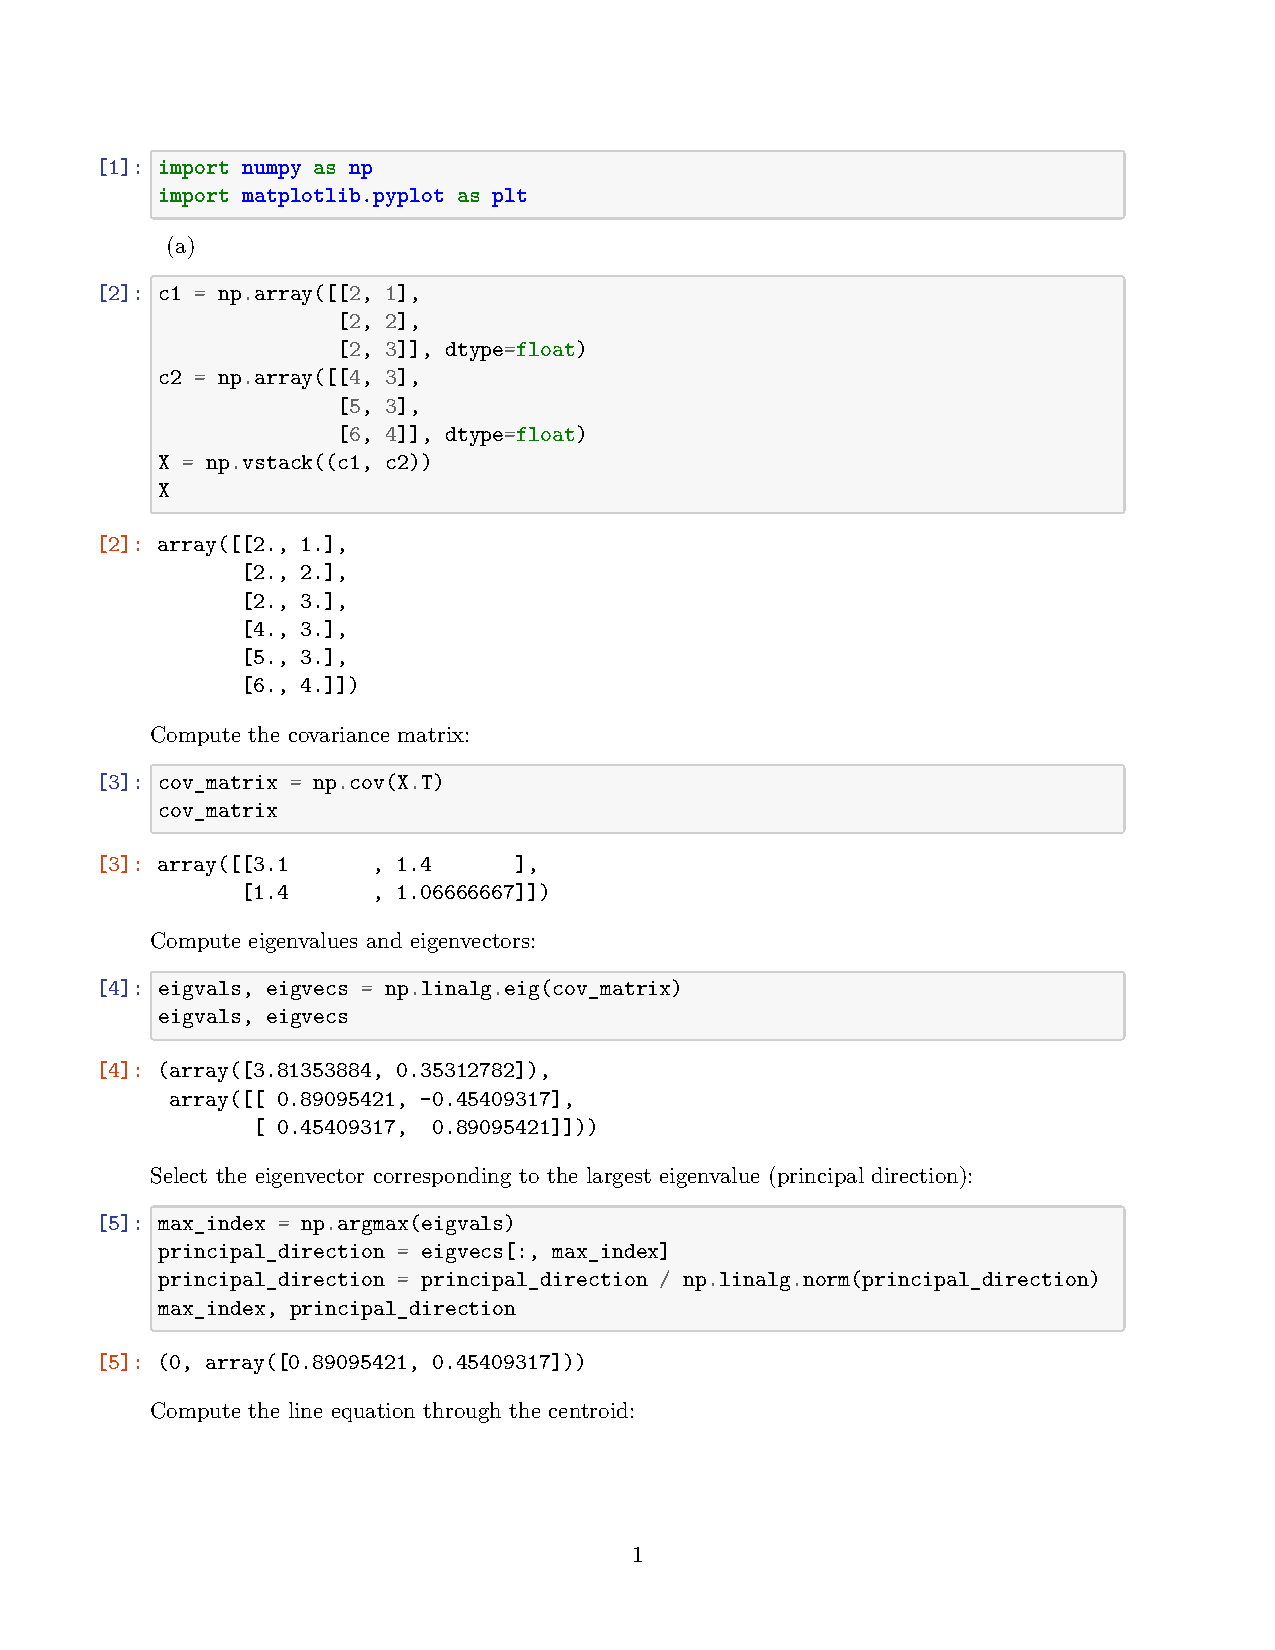
\includepdf[pages=-, scale=1]{Problem7/Problem7_1.pdf}
		
		\item[(2)] An alternative perspective on PCA views it as identifying the low-dimensional subspace that minimizes reconstruction error from dimensionality reduction. Remarkably, the variance-maximization and error-minimization objectives yield identical PCA solutions.
		
		\begin{enumerate}
			\item[(a)] Suppose all observations $\{\mathbf{x}_{1}, \dots, \mathbf{x}_{n}\}$ have been mean-centered. State the constrained optimization task for determining a direction vector $\mathbf{w}$ that defines a linear subspace minimizing the total squared reconstruction loss
			\[
			\sum_{i=1}^{n} d_{i}^{2}
			\]
			where $d_{i}$ quantifies the reconstruction discrepancy for $\mathbf{x}_{i}$, measured as the Euclidean distance from $\mathbf{x}_{i}$ to its orthogonal projection onto the subspace. Impose unit length constraint $\|\mathbf{w}\|=1$ since only direction matters. Express your objective solely using $\mathbf{w}$ and $\mathbf{x}_{i}$, eliminating $d_{i}$.
			
			\begin{your_solution}
				The dataset \(\{\mathbf{x}_1,\dots,\mathbf{x}_n\}\subset\mathbb{R}^d\) has been mean-centered, i.e. \(\sum_{i=1}^n\mathbf{x}_i=\mathbf{0}\). 
				
				We seek a unit-length direction vector \(\mathbf{w}\) (i.e. \(\|\mathbf{w}\|_2=1\)) that defines a one-dimensional linear subspace onto which we orthogonally project each \(\mathbf{x}_i\). 
				
				The orthogonal projection of \(\mathbf{x}_i\) onto span\(\{\mathbf w\}\) is \((\mathbf w^\top \mathbf x_i)\mathbf w\). 
				
				The squared reconstruction error for \(\mathbf x_i\) is therefore
				\[
				d_i^2 \;=\; \big\| \mathbf{x}_i - (\mathbf w^\top \mathbf{x}_i)\mathbf w\big\|_2^2.
				\]
				The total squared reconstruction loss over all samples is \(\sum_{i=1}^n d_i^2\). 
				
				Thus the constrained optimization problem (with the unit-norm constraint) is
				\[
				\boxed{ \;\min_{\mathbf w}\; \sum_{i=1}^n \big\| \mathbf{x}_i - (\mathbf w^\top \mathbf{x}_i)\mathbf w\big\|_2^2
				\quad\text{s.t.}\quad \|\mathbf w\|_2 = 1 \; }.
				\]

			\end{your_solution}
			\item[(b)] Using your formulation from (a), demonstrate that this minimization problem coincides with standard PCA when recognizing: 
			\[
			\Sigma = \sum_{i} \mathbf{x}_{i} \mathbf{x}_{i}^{T}
			\]

			\begin{your_solution}
				We'll prove that the above minimization is equivalent to maximizing \(\mathbf w^\top \Sigma \mathbf w\) where \(\Sigma=\sum_{i=1}^n \mathbf x_i\mathbf x_i^\top\).

				Start by expanding each term:
				\[
				\begin{aligned}
				\big\| \mathbf{x}_i - (\mathbf w^\top \mathbf{x}_i)\mathbf w\big\|_2^2
				&= (\mathbf{x}_i - (\mathbf w^\top \mathbf{x}_i)\mathbf w)^\top(\mathbf{x}_i - (\mathbf w^\top \mathbf{x}_i)\mathbf w) \\
				&= \left[\mathbf{x}_i^\top - w^\top(\mathbf{x}_i^\top \mathbf w)\right]\left[\mathbf{x}_i - (\mathbf w^\top \mathbf{x}_i)\mathbf w\right] \\
				&= \mathbf{x}_i^\top \mathbf{x}_i - 2(\mathbf w^\top \mathbf{x}_i)(\mathbf w^\top \mathbf{x}_i) + (\mathbf w^\top \mathbf{x}_i)^2(\mathbf w^\top \mathbf w) \\
				&= \|\mathbf{x}_i\|_2^2 - (\mathbf w^\top \mathbf{x}_i)^2,
				\end{aligned}
				\]
				where in the second line we used \(\mathbf w^\top\mathbf w = \|\mathbf{w}\|_2^2=1\). 
				
				Summing over \(i\) yields
				\[
				\sum_{i=1}^n d_i^2 \;=\; \sum_{i=1}^n \|\mathbf{x}_i\|_2^2 \;-\; \sum_{i=1}^n (\mathbf w^\top \mathbf{x}_i)^2.
				\]
				The first term \(\sum_i \|\mathbf{x}_i\|_2^2\) does not depend on \(\mathbf w\), so minimizing the left-hand side over unit \(\mathbf w\) is equivalent to maximizing the second term:
				\[
				\max_{\|\mathbf w\|=1} \; \sum_{i=1}^n (\mathbf w^\top \mathbf{x}_i)^2.
				\]
				Rewrite the objective in matrix form:
				\[
				\sum_{i=1}^n (\mathbf w^\top \mathbf{x}_i)^2
				= \sum_{i=1}^n \mathbf w^\top (\mathbf{x}_i\mathbf{x}_i^\top)\mathbf w
				= \mathbf w^\top \left(\sum_{i=1}^n \mathbf{x}_i\mathbf{x}_i^\top\right)\mathbf w
				= \mathbf w^\top \Sigma \mathbf w.
				\]
				Therefore the constrained minimization of total reconstruction error is equivalent to the Rayleigh quotient maximization
				\[
				\max_{\|\mathbf w\|_2 = 1} \; \mathbf w^\top \Sigma \mathbf w.
				\]
				By classical results, the maximizer is the eigenvector of \(\Sigma\) associated with the largest eigenvalue. This eigenvector is precisely the first principal component obtained by standard PCA (using \(\Sigma\) as the covariance matrix). Hence the reconstruction-error minimization formulation yields the same principal direction as the variance-maximization PCA formulation.

			\end{your_solution}
		\end{enumerate}
		
		
		\item[(3)] Acquire the MNIST handwritten digit dataset from \url{http://yann.lecun.com/exdb/mnist/}. Various Python utilities exist online for parsing the native format, or retrieve pre-processed Python-compatible data from \url{http://cs.nyu.edu/roweis/data.html}. You may use libraries such as \texttt{keras.datasets.mnist}, \texttt{torchvision.datasets.MNIST}, or\\ \texttt{sklearn.datasets.fetch\_openml} for convenient data loading.
		
		Develop your own PCA implementation without relying on pre-built library functions. You may utilize Python's built-in routines such as \texttt{numpy.linalg.svd} for SVD and \texttt{numpy.linalg.eig} (or \texttt{numpy.linalg.eigh} for symmetric matrices) for eigendecomposition. Include source code printout with your submission.
		
		Memory constraints: If computational resources prove insufficient, subsample to the first 1000 images per digit class. Should memory issues persist, further reduce to 100 images per class.
		
		
		\begin{enumerate}
			\item[(a)] Visualize the average digit-1 template and display the leading 5 principal components extracted from the complete dataset under two computational approaches: employing the Gram matrix technique versus the standard covariance approach.  
			Ensure mean-centering precedes PCA execution. Record computational time for principal component extraction in both scenarios. You may use \texttt{matplotlib.pyplot.imshow} for visualization and Python's \texttt{time} module (e.g., \texttt{time.time()}) for timing measurements.
			
			\item[(b)] Analyze the computational efficiency of each approach. Justify whether the Gram matrix strategy offers advantages for this specific dataset.
			
			\item[(c)] Select an arbitrary image (from any digit class) and transform it to the principal component basis (the global eigenspace from part (a)), then reconstruct using the leading $n$ components (cumulative up to $n$, not just component $n$) for both computational methods (Gram versus standard), with $n \in \{1, 2, 5, 10, 20\}$. Apply mean-centering before projection and restore the mean post-reconstruction.
			
			For each of the 5 reconstructions, quantify fidelity via mean squared error. The MSE metric for vectors $\mathbf{a}$ and $\mathbf{b}$ is 
			\[
			\text{MSE}(\mathbf{a}, \mathbf{b}) = \|\mathbf{a} - \mathbf{b}\|_{2}^{2}
			\]
			
			Present all reconstructions alongside the original in a composite figure, annotating each panel with its corresponding MSE. You may use \texttt{matplotlib.pyplot.subplot} to create composite figures and \texttt{numpy.linalg.norm} for computing Euclidean norms.
		\end{enumerate}

		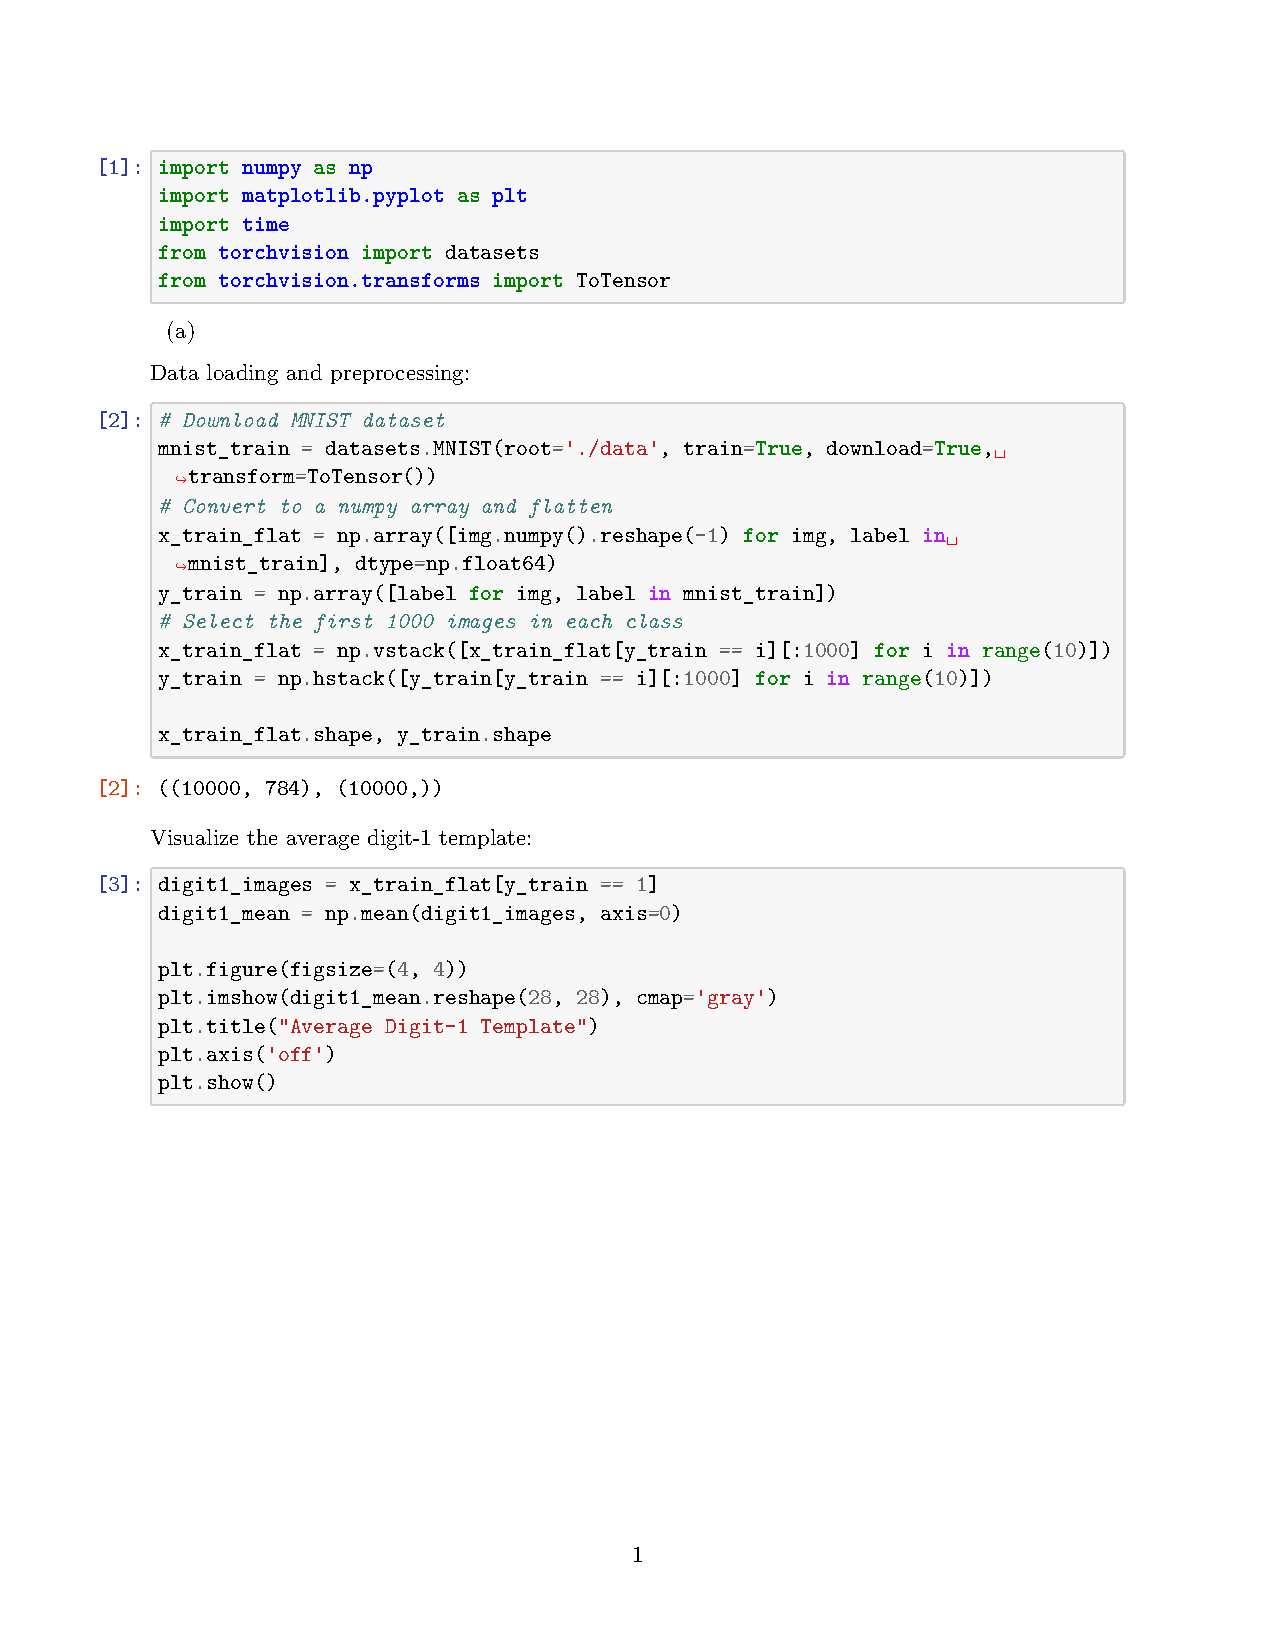
\includepdf[pages=-, scale=1]{Problem7/Problem7_3.pdf}
		
	\end{enumerate}
	
	\clearpage
	
	
\end{document}